\documentclass[10pt, twopage headsepline]{manual}
\usepackage{computer-manual}
\makeindex

\title{Tellervo}
\subtitle{A guide for users and developers}
\authors{Peter W.\ Brewer}
\version{1.0}

%% Define the path to the resources folder so that we can
%% seamlessly use application images/icons in document
\graphicspath{{../src/main/resources/}}

\begin{document}

  \begin{titlepage}
\AddToShipoutPicture*{\BackgroundPic}

%{ 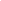
\includegraphics{Images/pixel.png}\\[2cm] 
%\raggedleft

%\Huge \bfseries \textcolor{white}{\hrule 
%\vspace{5mm}CORINA MANUAL}\\[3mm] 
%\large{\textcolor{white}{For users and developers
%\vspace{5mm}
%\hrule}}

%\vspace{3cm}
%}

%{
%\normalsize
%\raggedleft\textbf{\textcolor{white}{By Peter W.\ Brewer and Ken Harris}}\\[0.6cm]
%}
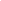
\includegraphics{Images/pixel.png}\\[187mm] 
{
\raggedleft
\Large \textbf{By \authornames}\\
}

\vfill
{
\large For Corina server and desktop\\
version \versionnumber\\[2mm]
\today\\[2mm]
}


%{\footnotesize
%\textcolor{white}{Corina was developed by Peter Brewer, Chris Dunham, Aaron Hamid, Ken Harris, Drew Kalina, Lucas Madar, Daniel Murphy, Robert 'Mecki' Pohl and Kit Sturgeon}
%}
%{\normalsize Cornell Tree-Ring Laboratory\\B48 Goldwin Smith Hall\\Cornell University\\Ithaca NY 14853. USA}

\end{titlepage}
  


\thispagestyle{empty} 
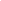
\includegraphics{Images/pixel.png}
\vfill
\parbox[b]{11cm}{\raggedright

\textcopyright {\the\year} Peter W. Brewer\\[2mm] Malcolm and Carolyn Wiener Laboratory for Aegean\\ and Near Eastern Dendrochronology \\
Cornell Tree-Ring Laboratory\\
B48 Goldwin Smith Hall\\ Cornell University \\ Ithaca, New York 14853. USA.\\[0.5cm] \Telefon\hspace{3mm}+1 607 255 8650 \\ \Letter\hspace{3mm}p.brewer@cornell.edu\\[5mm] Compiled: \today\\[10mm]}

{\footnotesize 
Permission is granted to copy, distribute and/or modify this document
under the terms of the GNU Free Documentation License, Version 1.3
or any later version published by the Free Software Foundation;
with no Invariant Sections, no Front-Cover Texts, and no Back-Cover Texts.
A copy of the license is included in the appendix entitled ``GNU Free Documentation License'' (pages \pageref{txt:FDLStart}--\pageref{txt:FDLEnd}).}



\newpage
\pagenumbering{roman}
\setcounter{page}{1}
\thispagestyle{empty} 
{ 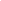
\includegraphics{Images/pixel.png}\\[4cm] 
\hrule 
\vspace{5mm}
\Huge \bfseries \thetitle\\[3mm] 
\large{\thesubtitle}
\vspace{5mm}
\hrule
\vspace{3cm}
}
{
\normalsize
\textbf{By \authornames}\\[0.6cm]
}
{
\vfill
\footnotesize
Compiled: \today
}

\newpage


\tableofcontents


\cleardoublepage
\pagenumbering{arabic} 

\phantomsection
\section*{Preface}
\thispagestyle{empty} 
\addcontentsline{toc}{section}{Preface}

Tellervo\footnote{The name Tellervo is derived from the Finnish goddess of the forest.} is primarily focused on the measurement of tree ring widths and the organization and curation of the data, metadata and physical samples for dendrochronolgoical research. It is cross-platform (running on all Java 6 enabled operating systems including Windows, MacOSX and Linux) and open-source. It includes support for standard measuring platforms including Velmex, Lintab and Henson.

Tellervo is an extension of the original application `Corina' developed at Cornell University since 2000.  Corina itself following an earlier DOS-based version programmed in C, which in turn was derived from a collection of FORTRAN and C utilities.  Corina is built around a standard file-based data management system. In 2007, work began on a major rewrite of the software whereby this file-based data management was replaced with an object-relational database management system (ORDBMS) and server/client webservice infrastructure.  The application was renamed Tellervo to reflect the substantial changes made from the original Corina code-base.

The Tellervo initiative was made possible because of the support of the College of Arts \& Sciences, Cornell University, via a grant to Sturt Manning to re-envisage the Cornell Tree-Ring Laboratory.

This manual is divided into two main sections, the first for users, the second for developers.  Tellervo is open source software (see the details of the license on pages \pageref{txt:licenseStart}--\pageref{txt:licenseEnd}), so you are welcome to inspect and edit the code.  The second part of this manual will help you do that.

Over the years Corina and Tellervo have been developed by a number of people: Peter Brewer, Chris Dunham, Aaron Hamid, Dan Girshovich, Ken Harris, Drew Kalina, Rocky Li, Lucas Madar, Daniel Murphy, Robert 'Mecki' Pohl and Kit Sturgeon.  We would like to thank the many people that have tested the applications especially: Charlotte Pearson; Carol Griggs; Brita Lorentzen; Jess Herlich; LeAnn Canady; Kate Seufer; and many undergraduate and postgradutes students at Cornell.  

We would also like to thank the College of Arts \& Sciences and the Department of Classics, Cornell University; the Malcolm H.\ Wiener Foundation; and the many patrons of the Malcolm and Carolyn Wiener Laboratory for Aegean and Near Eastern Dendrochronology for their financial support.  

We hope that you find Tellervo useful and look forward to hearing your feedback.  





  %%%%%%%%%%%%
  \part{User Guide}
  %%%%%%%%%%%%
    
\chapter{Installation}

Corina is made up of two packages; the Corina desktop application and the Corina database server.  Corina was designed primarily for laboratories with multiple users, each running the Corina desktop application on their own computer connecting to a single central server containing the lab's data.  In this situation the Corina server would be run on a separate computer to those running the desktop client, but this need not necessarily be the case.  It is perfectly possible to run both the server and the client on the same computer.  This is likely to be the situation if you simply want to try out Corina, if you don't have a separate server, or if you do not work in a multi-user laboratory.


\section{Desktop application}

Installation packages for the Corina desktop application are available for Windows, MacOSX and Ubuntu Linux.  Corina can also be run on other operating systems as long as they support Java 6.

To install Corina, download the installation file for your operating system from \url{http://dendro.cornell.edu/corina/download.php}. The website should provide you with a link to the installer for your current operating system:

\begin{description}
\item 
\includegraphics[width=3mm]{Images/windows.png} \textbf{Windows} -- Run the setup.exe and follow the instructions. If you do not have Java installed the installer will direct you to the Java website where you can get the latest version. Once installed, Corina can be launched via the Start menu.

\item 
\includegraphics[width=3mm]{Images/mac.png} \textbf{Mac OS X} -- As mentioned above, Corina requires Java 6. Although MacOSX ships with Java installed, unfortunately Apple have been very slow to provide Java 6. Although it was released in 2006, it was not until August 2009 that Apple made Java 6 available as part of v10.6 (snow leopard). Corina can therefore only be run on Snow Leopard or later. To do so, download the dmg disk image file and mount it by double clicking on it. Drag the Corina.app into your applications folder and copy the manual and license files to somewhere convenient in your documents folder.  For the more adventurous there is the possibility that you could run Corina using SoyLatte instead of the standard Java installation that comes with the operating system.  This could be a possible method for running Corina even on earlier versions of MacOSX but is unsupported and largely untested.

\item 
\includegraphics[width=3mm]{Images/ubuntu.png} \textbf{Ubuntu Linux} --  A deb file is available which was designed for use on Ubuntu distributions but should work on any Debian based system. Install using your favorite package management system e.g. \verb|sudo dpkg --install corina\_2.xx-1\_all.deb|. On Ubuntu and similar distributions, the package should add a Corina shortcut to your applications menu. Alternatively you can start Corina from the command line by typing corina.

\item 
\includegraphics[width=3mm]{Images/java.png} \textbf{Other operating systems} -- Make sure you have Java 6 installed, then download the Corina jar file to your hard disk. You can run Corina from the command line by typing: \verb|java -jar corina.jar|.
\end{description}

\subsection{Mapping support}

Corina includes 3D mapping for visualization of sampling locations. Although this is not necessary for most tasks, to make use of the mapping functions you will require a OpenGL 3D capable graphics card. To check whether your computer already supports 3D mapping, open Corina, go to Admin, then Site map.  Corina will warn you if your graphics card is not supported.

All MacOSX computers should automatically support OpenGL.  Most Windows and Linux computers made since 2006 should also support OpenGL, however, this does require proper drivers to be installed. In some cases Windows computers may include a compatible graphics card, but may only have the default Windows video drivers installed.  If you are having trouble with the mapping in Corina make sure you have installed the most recent drivers for your graphics card.  Linux users may be required to install proprietary graphics drivers.  

The mapping component of Corina makes use of NASA's open source World Wind Java.  NASA's website \url{http://worldwind.arc.nasa.gov/} contains further information and instructions that you may find helpful if you are having problems getting the mapping to work.  

\section{Server installation}

For the Corina desktop application to be useful you will also require access to a Corina server.  If you are running Corina in a lab where the Corina server has already been set up by your systems administrator, you can skip this section.

The Corina server is made up of a number of components, which unlike the desktop client, can not be easily combined together into cross-platform packages.  Although all the constituent components are open-source and available for all major platforms, building and maintaining separate packages for each platform is too large a task for a small development team.  To conserve resources, we therefore made the decision to utilize Virtual Machine technology to ensure that the Corina server could still be run on all major operating systems.  This means that we can package the Corina server for a single operating system (Ubuntu Linux) and then distribute it as a Virtual Appliance that can be run as a program on your normal operating system. 

The Corina server is therefore available via two main methods.  The first is as a VirtualBox Virtual Appliance which can be run on any major operating system, the second is as an Ubuntu package for running natively on a Linux server.  The source code for the server is also available so it is perfectly possible for more experienced users to set up the Corina server to run natively on other platforms.  For this you will require knowledge of Apache 2, PHP and PostgreSQL.

\subsection{Virtual Appliance - all operating systems}

To run the Corina server Virtual Appliance, you will first need to download and install VirtualBox from \url{http://www.virtualbox.org}.  Installation packages are available for Windows, MacOSX, OpenSolaris and many Linux distributions.

Once you have VirtualBox installed, you will then need to download the Corina server from the Cornell website \url{http://dendro.cornell.edu/corina}.  This package contains a bare-bones Ubuntu Linux server with everything required to run the Corina server installed and ready to use.  As VirtualBox, the entire Ubuntu operating system and Corina server components are all open source there are no license fees to pay.

Open VirtualBox and go to File, Import Appliance, then follow the wizard selecting the Corina server appliance file when prompted.  Once installed you can run your server by highlighting it in the list and pressing start.  The server will boot up in a window alongside your normal operating system and eventually reach a login prompt.  To save on download size and disk space only the essential packages to make the server run have been installed.  This means there is no graphical interface just a command line.  Hopefully this should not be a problem as once set up, the only interaction needed with the Virtual Appliance will be through the normal Corina desktop application.  If you would prefer to use a graphical interface to the server this can be easily installed.  See chapter \ref{txt:servermaintenance} for further details.latex define environment

Before you can use your server you will need to know the IP address that the server has been assigned by your network.  To do this login at the prompt with the default admin credentials: user -- corina; password -- w3l0v3tr33s.  Once logged in, type \verb|corina --test| and a basic configuration test will be performed.  If all is well, all tests will be passed and it will tell you the URL of your new server.  You will need to set your Corina client to point at this webservice to use your server.



\subsection{Ubuntu native installation}

If you are fortunate enough to be running Ubuntu then the native Ubuntu deb package is the best and easiest method for installing the Corina server, otherwise see section \ref{txt:virtualAppliance} to install the server as a Virtual Appliance.  

To install the Corina server in Ubuntu simply download the deb package from the Cornell server \url{http://dendro.cornell.edu/corina} and install with your favourite package manager.  For instance, to install from the command line simply type \verb|sudo dpkg --install corina-server.deb|. The package will automatically run a configuration script to assist with creating a database user, building the Corina PostgreSQL database, setting database permissions and setting up the Apache webservice.  The configuration ends with a test routine to check all services are set up correctly and if so, will provide you with the URL of the newly configured Corina webservice.

\subsection{Advanced install on other operating systems}

As mentioned previously, the limited resources available for Corina development means that we have been unable to produce native installers for platforms other that Ubuntu.  If you are an experience systems administrator though, it should not be too difficult to set up the Corina server manually.  

The Corina server is essentially a PostgreSQL database accessed via a PHP webservice running on Apache 2.  The following dependencies are therefore required: postgresql-8.4; postgis; postgresql-contrib-8.4; postgresql-8.4-pljava; sun-java6-jre; apache2; php5; php5-pgsql; php5-curl; php5-mhash.

The basic procedure for installation is as follows:

\begin{itemize*}
 \item Install all dependencies
 \item Create PostgreSQL database from Corina template SQL file
 \item Set up a database user and provide access to the server in the pg\_hba.conf file
 \item Give this user read and write permissions to the database
 \item Copy the webservice code into a web accessible folder
 \item Set up Apache to see this folder by creating an entry in the sites-enabled folder
 \item Restart PostgreSQL and Apache and check you can access the webservice from a web browser
\end{itemize*}


    
\chapter{Getting started}






    %\chapter{Measuring samples}

Although it is possible to manually enter the ring widths of your samples into Corina, it is normal to automate this process using a measuring platform. Corina supports the most common measuring platforms including Velmex and Lintab.

\section{Configuring measuring platforms}

Measuring platforms typically use serial ports to communicate to computers. In recent years computer manufacturers have been phasing out serial ports so you may need to purchase a serial-USB converter. Modern MacOSX, Linux as well as Windows 7 should support most serial-USB adapters out of the box, otherwise you must install the relevant drivers before continuing.  Recent Lintab USB platforms use internal seriesl-USB converters so are treated in exactly the same way by Corina.

To begin, shut down your computer, attach your platform, then reboot and launch Corina. Next, go to the preferences window and open the hardware tab and you should see an interface that looks like figure \ref{fig:hardwareprefs}.

\begin{figure}[hbtp]
  \centering
    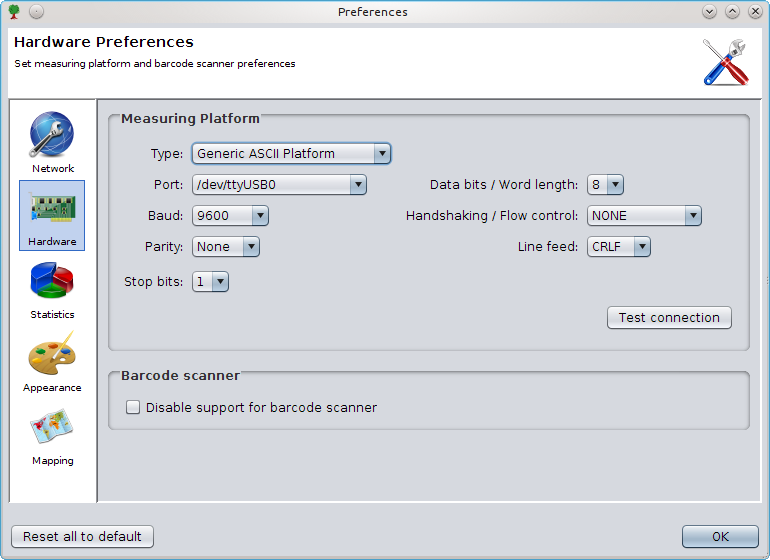
\includegraphics[width=0.6\textwidth]{Images/hardwareprefs.png}
    \caption{The hardware preferences dialog.}
    \label{fig:hardwareprefs}
\end{figure}


In the type pull down menu, select the type of measuring equipment you are using. Note that this refers to the equipment that the computer is attached to, and not necessarily the measuring platform itself. For instance, Velmex platforms are typically connected through a Metronics digital readout device. Included in this list is the EveIO device which is an open-source device designed for the Cornell Tree-Ring Laboratory. Circuit drawings for this device can be obtained from the Cornell lab to enable Hensen measuring platforms to be used with Corina (and other software).

\info{Standard Lintab platforms use a proprietary communications protocol. Rinntech--the manufacturers of Lintab platforms--claim intellectual property rights over this protocol. During discussions between the Corina development team and Rinntech an agreement was reached whereby the Corina developers agreed not to release details of the protocol. In turn Rinntech has agreed to produce an adapter that can be attached to Lintab platforms so that they communicate with an open ASCII protocol. Users wishing to use Lintab platforms with Corina (or any software not developed by Rinntech) must therefore contact Rinntech and purchase an adapter.}

Next you must choose the port that your platform is connected to from the pull down menu. In Windows this will be a COM port, in Linux and Mac this will be a /dev/xxx port.  Depending on the type of platform you choose, you may also need to set various communication parameters.  If these boxes are enabled, please check the documentation that came with your measuring platform to ensure these values are set correctly.

To check whether your platform is working, click the `Start measuring test' button and attempt to measure a few rings.  Once you are satisfied, click OK on the preferences window and you will be returned to the Corina home screen.

\section{Differences in measuring hardware}

Different measuring platforms have different capabilities.  For instance, some include a physical switch for firing measurement events, others also include switches for resetting measurements to zero.  Some platforms (e.g. Lintab) also continuously report the measurement values to the computer.  So depending on the hardware you use, Corina will present the you with slightly different options.  

Please note that the architecture of Corina is such that providing support for additional measuring platforms is a relatively simple task.  If you have equipment that is not currently supported, please contact the developers to see if it can be included.  


\section{Measuring a sample}

Once your measuring platform has been configured, measuring your first sample is simple.  To start a new measurement go to File \MVRightarrow New or click the `new' icon on the home screen. A dialog will appear where you can scan your sample's barcode, or press the button to enter metadata for your sample later. Barcodes minimize data entry errors and also speed up the process of measuring your samples. See section \ref{txt:barcode} for more information. Once you have scanned your barcode or pressed the button, you will then be presented with an empty Corina data screen (figure \ref{fig:datascreen}).

\begin{figure}[hbtp]
  \centering
    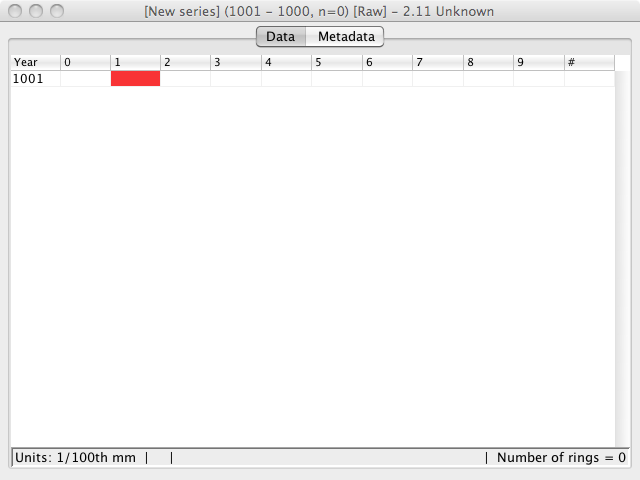
\includegraphics[width=0.6\textwidth]{Images/datascreen.png}
    \caption{An empty data window ready to receive measurements.  Note the status bar at the bottom includes buttons for changing the display units and cumulative statistics.}
    \label{fig:datascreen}
\end{figure}

The next step is to fill out the metadata tab. If you have used a barcode, nearly all of this metadata will be filled in for you, otherwise you will need to fill this out yourself. Details about metadata can be found in chapter \ref{txt:metadata}, page \pageref{txt:metadata}.

To begin measuring your sample you can now go to Edit \MVRightarrow Start measuring or you can press F5. While measuring you should be provided with audible feedback for each ring measured with a more pronounced sound made every 10th ring. If there is a problem communicating with your measuring hardware, check your settings in the preferences dialog. If you still have problems contact the Corina developers by going to Help \MVRightarrow Report bug on last transaction, making sure you include your email address and any further information.

While you measure your sample you can flag features in a ring by right clicking on any cell in the table and selecting one or more of the standard notes (see figure \ref{fig:ringremarks}).  

\begin{wrapfigure}{r}{0.5\textwidth}
  \begin{center}
    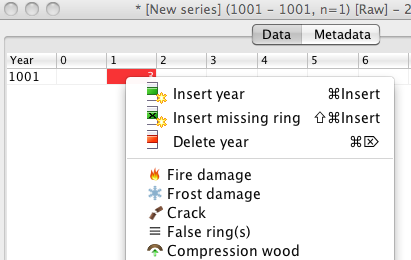
\includegraphics[width=0.48\textwidth]{Images/ringremarks.png}
  \end{center}
  \caption{Right click context menu showing some of the options for adding remarks to rings.}
  \label{fig:ringremarks}
\end{wrapfigure}

Corina supports all standard TRiDaS remarks including: fire damage; frost damage; crack; false ring(s); compression wood; tension wood; traumatic ducts; single pinned; double pinned; triple pinned and many others.  Rings that include remarks are indicated by the relevant icon in the data screen.  Depending on your method of work, this can be useful for keeping track of sample pin holes.  For instance, if a missing or false ring is discovered after a sample has been pinholed, the offset in pinholes can be easily seen without resurfacing the sample.  In the future Corina will also include support for user defined ring remarks.  

The data screen also contains a status bar at the bottom. By click on the units section, you can switch between micron and 1/100th mm units. Corina understands the units being supplied by the measuring platform, therefore changes here are purely for display purposes only. If you have a platform that measures in microns, but prefer to see the values in 1/100th mm then you can use this feature. At the bottom ring of the status bar you can choose one of a variety of summary information about your series.

Once you have finished measuring your sample, you should then go to File \MVRightarrow Save to save your series to the database. 
    \chapter{Measuring platforms}
\label{txt:MeasuringPlatformConfig}
\index{Measuring platforms}
\index{Hardware|see{Measuring platforms}}

Although it is possible to manually enter the ring widths of your samples into Tellervo, it is normal to automate this process using a measuring platform. Tellervo supports the most common measuring platforms including Velmex and Lintab.  However, please note that standard Lintab platforms use a proprietary communications protocol. Rinntech--the manufacturers of Lintab platforms--claim intellectual property rights over this protocol. During discussions between the Tellervo development team and Rinntech an agreement was reached whereby the Tellervo developers agreed not to release details of the protocol. In turn Rinntech has agreed to produce an adapter that can be attached to Lintab platforms so that they communicate with an open ASCII protocol. Users wishing to use Lintab platforms with Tellervo (or any software not developed by Rinntech) must therefore contact Rinntech and purchase an adapter.

Measuring platforms typically use serial ports to communicate to computers. In recent years computer manufacturers have been phasing out serial ports so you may need to purchase a serial-USB converter. Modern MacOSX, Linux as well as Windows 7 should support most serial-USB adapters out of the box, otherwise you must install the relevant drivers before continuing.  Recent Lintab USB platforms use internal serial-USB converters so are treated in exactly the same way by Tellervo.

To begin, shut down your computer, attach your platform, then reboot and launch Tellervo. Next, go to the preferences window and open the hardware tab and you should see an interface that looks like figure \ref{fig:hardwareprefs}.

\begin{figure}[hbtp]
  \centering
    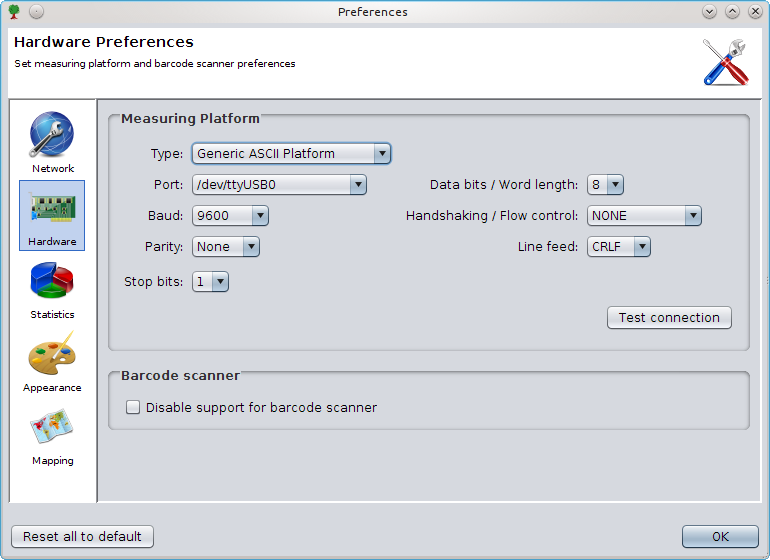
\includegraphics[width=0.6\textwidth]{Images/hardwareprefs.png}
    \caption{The hardware preferences dialog.}
    \label{fig:hardwareprefs}
\end{figure}

In the type pull down menu, select the type of measuring equipment you are using. Note that this refers to the equipment that the computer is attached to, and not necessarily the measuring platform itself. For instance, Velmex platforms are typically connected through a Metronics digital readout device. Included in this list is the EveIO device which is an open-source device designed for the Cornell Tree-Ring Laboratory. Circuit drawings for this device can be obtained from the Cornell lab to enable Hensen measuring platforms to be used with Tellervo (and other software).  If you measuring platform is not included in the list it should be relatively easy for us to add support so please get in touch and we'll see what we can do.  Alternatively you could implement support yourself (either personally or by employing an independent developer).  Technical details on how to do this are included in section \ref{txtSupportingNewMeasuringPlatforms}, page \pageref{txtSupportingNewMeasuringPlatforms}.  

Next you must choose the port that your platform is connected to from the pull down menu. In Windows this will be a COM port, in Linux and Mac this will be a /dev/xxx port.  Depending on the type of platform you choose, you may also need to set various communication parameters.  If these boxes are enabled, please check the documentation that came with your measuring platform to ensure these values are set correctly.

To check whether your platform is working, click the `Test connection' button (see figure \ref{fig:hardwaretest}) and attempt to measure a few rings.  Different measuring platforms have different capabilities.  For instance, some include a physical switch for firing measurement events, others also include switches for resetting measurements to zero.  Some platforms (e.g. Lintab) also continuously report the measurement values to the computer.  So depending on the hardware you use, Tellervo will present the you with slightly different options.  

\begin{wrapfigure}{r}{0.5\textwidth}
  \begin{center}
    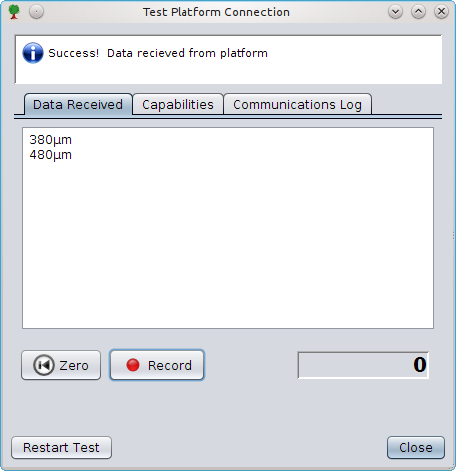
\includegraphics[width=0.48\textwidth]{Images/hardwaretestdialog.png}
  \end{center}
    \caption{Testing the connection to a hardware measuring platform.}
    \label{fig:hardwaretest}
\end{wrapfigure}



The test dialog includes information about the capabilities of your platform as well as a log window to show the raw information being received by Tellervo.  If you are having trouble interfacing with your platform, you should send the communications log to the developers, along with as much information about your hardware as possible.

Once you are satisfied that you are getting the correct results from the measuring platform, click close on the test window and then close the preferences dialog to return to the Tellervo home screen.






    \chapter{Metadata}
\label{txt:metadata}
\index{Metadata|(}
Metadata is `data about data'. In Tellervo this means all the information associated with your physical samples and measurement series e.g. species, location, who measured it, dimensions, slope, soil type etc.

The metadata in Tellervo, and in fact the entire Tellervo data model, is based on the Tree Ring Data Standard (TRiDaS). Before you use Tellervo you may find it useful to read \citet{tridas} so that you get a better understanding of the principles of TRiDaS, but a summary is also provided here.

\section{Tree Ring Data Standard - TRiDaS}
\index{TRiDaS|textbf}
TRiDaS is an XML-based data standard for recording dendrochronological data and metadata. More than 80 dendrochronologists, computer scientists and specialists from research disciplines that rely on dendrochronology have so far contributed to its development, including dendroarchaeologists, art and architecture historians, ecologists, geologists and climatologists.  The standard is therefore capable of recording the wide variety of metadata required by these different fields. TRiDaS builds upon other established standards, such as GML for the recording of locality information.  The extensible nature of XML also means that TRiDaS can evolve to accommodate the changing needs of dendrochronologists over time.  

TRiDaS includes a total of eight data entities: project; object; element; sample; radius; measurementSeries; derivedSeries; and value.  Detailed descriptions of each of these entities are given below and their relationships are illustrated in figure \ref{fig:datamodel}.

\begin{figure}
\centering
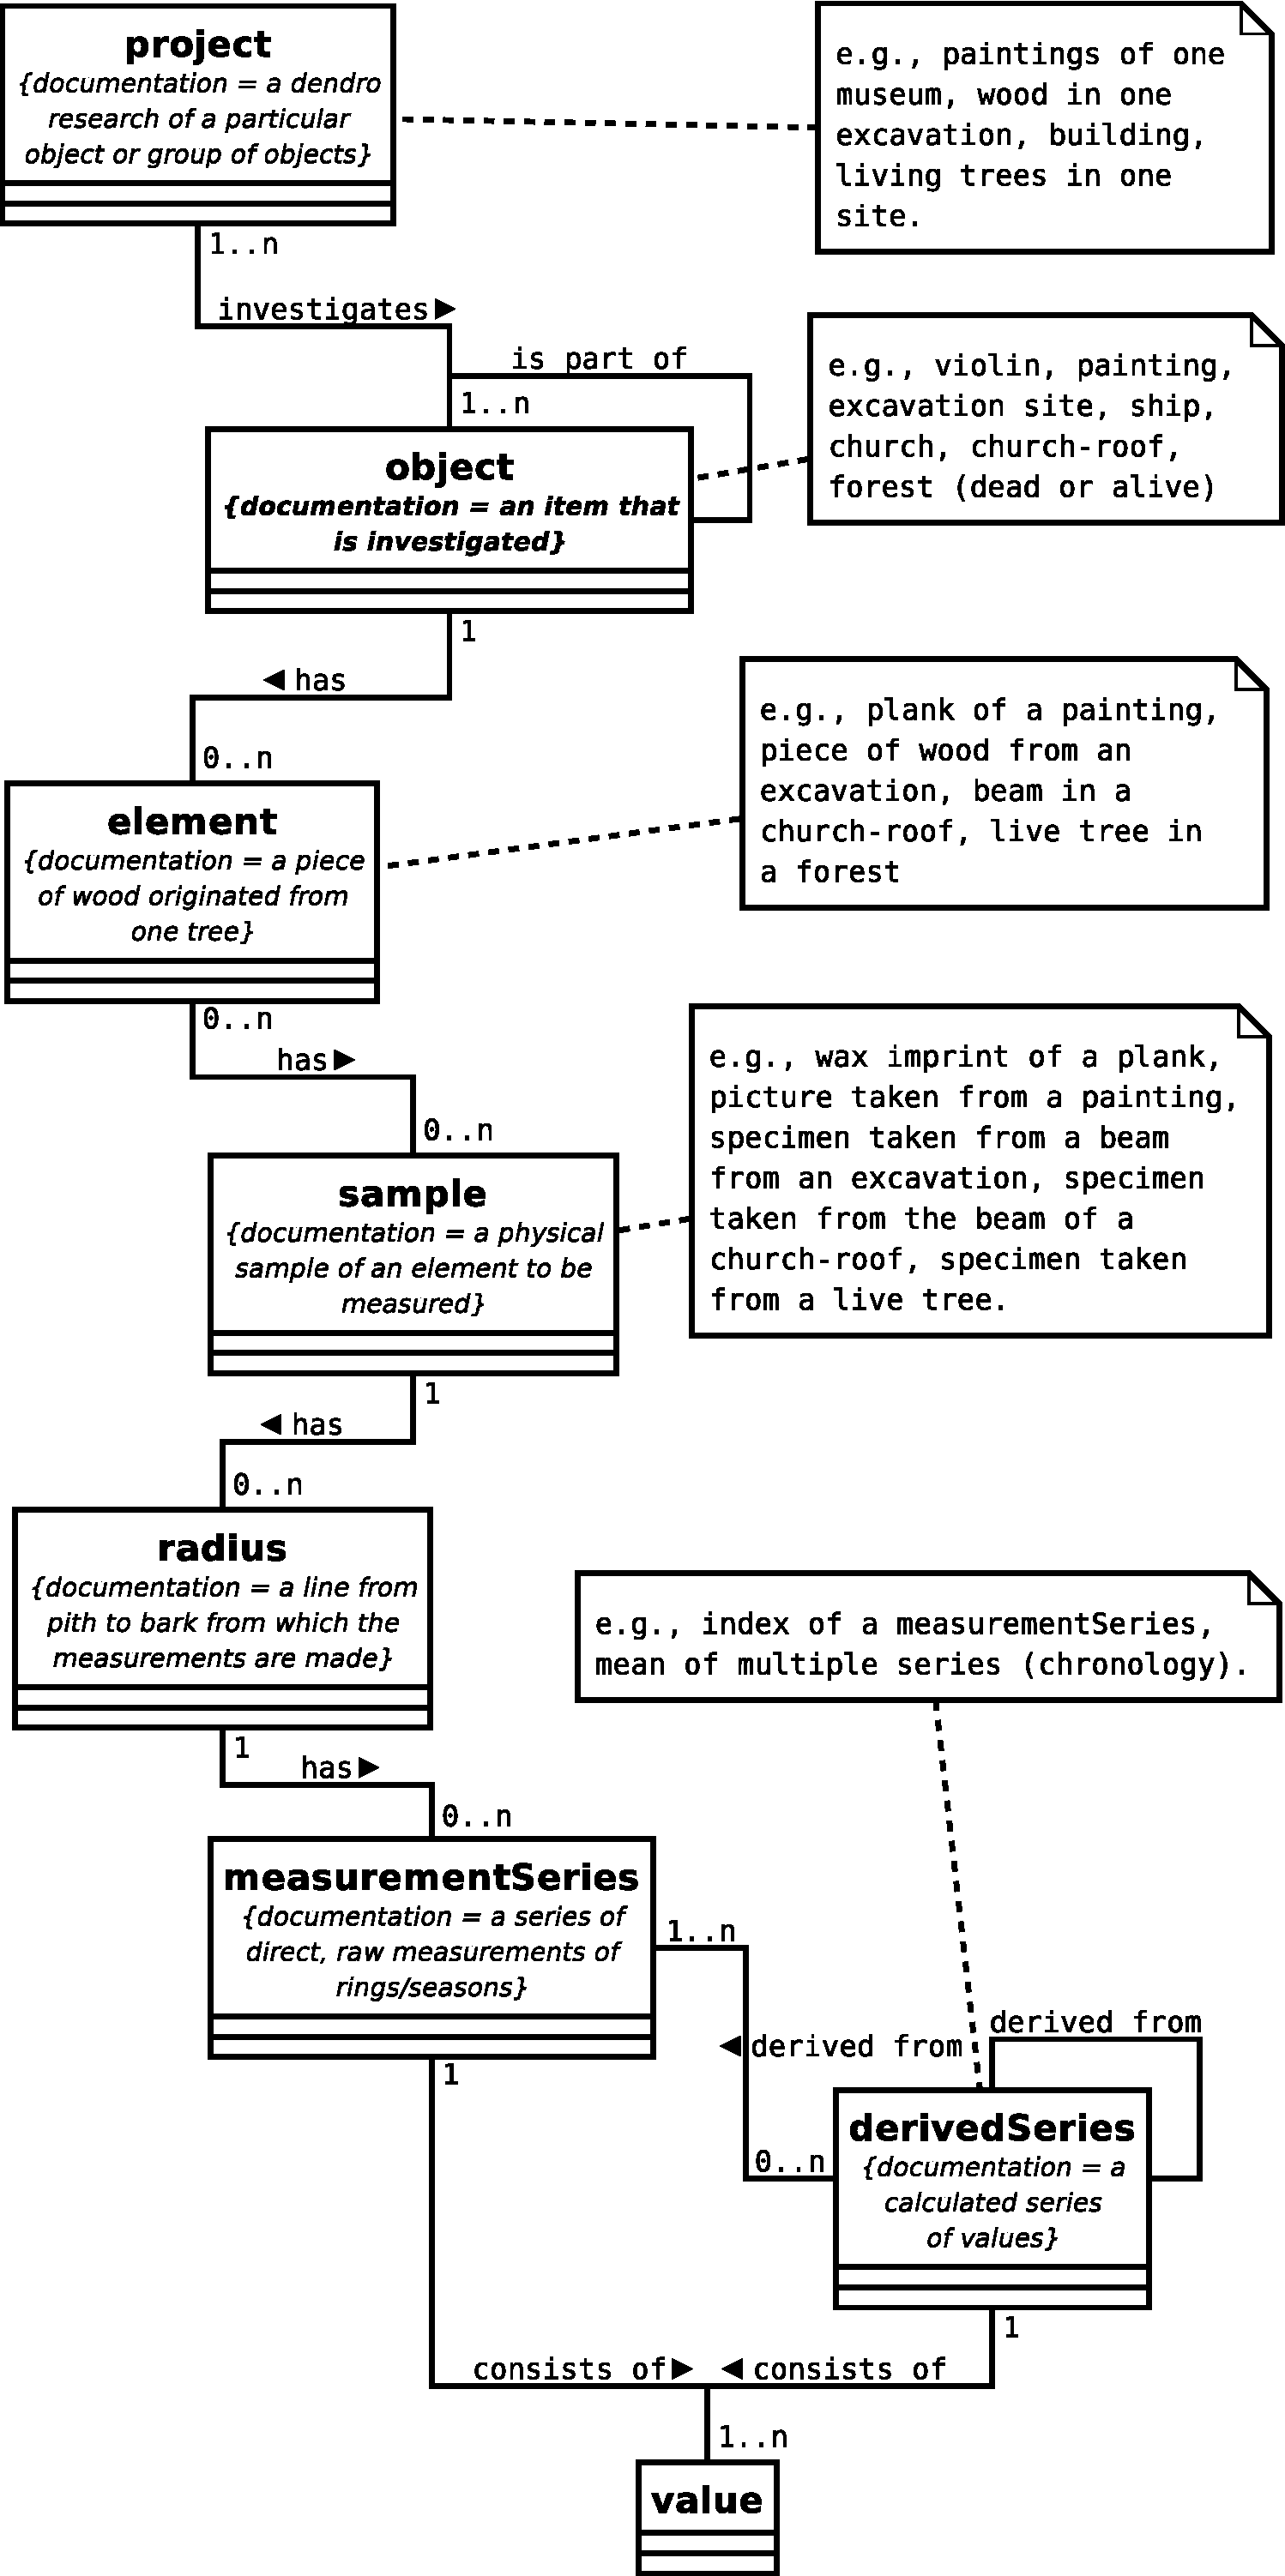
\includegraphics[height=0.9\textheight]{Images/datamodel.pdf}
\caption{TRiDaS data model showing the relationships between data entities.  Most of the entities having a simple hierarchical relationship (a project has one or more objects, an element has one or more samples.} 
\label{fig:datamodel}
\end{figure}

\begin{description}

\item 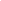
\includegraphics[width=5mm]{Images/pixel.png}  \textbf{A project} -- is defined by a laboratory and encompasses dendrochronological research of a particular object or group of objects.  Examples include: the dating of a building; the research of forest dynamics in a stand of living trees; the dating of all Rembrandt paintings in a museum. What is considered a ``project'' is up to the laboratory performing the research. It could be the dating of a group of objects, but the laboratory can also decide to define a separate project for each object. Therefore, a project can have one or more objects associated with it.  Due to the way research is conducted at the Cornell Tree-Ring Lab, TRiDaS projects are not currently supported within Tellervo, although future plans include adding project support.

\item 
\includegraphics[width=5mm]{Icons/128x128/object.png} \textbf{An object} -- is the item to be investigated.  Examples include: violin; excavation site; painting on a wooden panel; water well; church; carving; ship; forest. An object could also be more specific, for example: mast of a ship; roof of a church. Depending on the object type various descriptions are made possible. An object can have one or more elements and can also refer to another (sub) object.  For instance a single file may contain three objects: an archaeological site object, within which there is a building object, within which there is a beam object.  The list of possible object types is extensible and is thus flexible enough to incorporate the diversity of data required by the dendro community.  Only information that is essential for dendrochronological research is recorded here. Other related data may be provided in the form of a link to an external database such as a museum catalogue. 

\item 
\includegraphics[width=5mm]{Icons/48x48/element.png} \textbf{An element} -- is a piece of wood originating from a single tree. Examples include: one plank of a water well; a single wooden panel in a painting; the left-hand back plate of a violin; one beam in a roof; a tree trunk preserved in the soil; a living tree. The element is a specific part of exactly one object or sub object.  An object will often consist of more than one element, e.g., when dealing with the staves (elements) of a barrel (object).  One or more samples can be taken from an element and an element may be dated using one or more derivedSeries.

\item 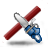
\includegraphics[width=5mm]{Icons/48x48/sample.png} \textbf{A sample} -- is a physical specimen or non-physical representation of an element. Examples include: core from a living tree; core from a rafter in a church roof; piece of charcoal from an archaeological trench; slice from a pile used in a pile foundation; wax imprint of the outer end of a plank; photo of a back plate of a string instrument. Note that a sample always exists and that it can either be physical (e.g.\ a core) or representative (e.g.\ a picture). A sample is taken from exactly one element and can be represented by one or more radii.

\item 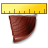
\includegraphics[width=5mm]{Icons/48x48/radius.png} \textbf{A radius} --  is a line from pith to bark along which the measurements are taken. A radius is derived from exactly one sample. It can be measured more than once resulting in multiple measurementSeries.

\item 
\includegraphics[width=5mm]{Icons/48x48/measurementseries.png} \textbf{A measurementSeries} -- is a series of direct, raw measurements along a radius. A single measurementSeries can be standardised or a collection of measurementSeries can be combined into a derivedSeries.  The measurements themselves are stored separately as values.

\item 
\includegraphics[width=5mm]{Icons/48x48/derivedseries.png} \textbf{A derivedSeries} -- is a calculated series of values and is a minor modification of the ``v-series'' concept proposed by \cite{corina}.  Examples include: index; average of a collection of measurementSeries such as a chronology. A derivedSeries is derived from one or more measurementSeries and has multiple values associated with it.

\item 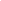
\includegraphics[width=5mm]{Images/pixel.png} \textbf{A value} --  is the result of a single ring measurement. Examples include: total ring width; earlywood width; latewood width. The values are related to a measurementSeries or a derivedSeries. In case of a measurementSeries the variable and its measurement unit (e.g.\ microns, 1/100th mm etc) are recorded as well.  Tellervo currently only supports total ring width values.  Support for other variables is planned for a future version.

\end{description}


Working top to bottom, the TRiDaS entities are nested within each other.  For instance a project contains one or more objects, which in turn contains one or more elements, and so on.  The benefit of this is that you record data once and once only.  In standard file-based dendrochronological software, when creating measurement series you are typically required to type the name of the site, the species of tree etc over and over again.  This is not only time consuming, but very error prone.  

Keeping data consistent is also difficult.  For instance, if it was determined that a tree species was identified incorrectly, in existing file-based software, the user would need to locate all data series from this tree and manally update the metdata.  This is not the case in Tellervo.  A tree is represented just once in Tellervo and samples of this tree, and the subsequent measurement series reference this one entry.  If metadata for this tree needs to be changed, the tree record is updated in just this one place.  Because the measurement series obtain this information by reference, then all associated series are automatically kept up to date.

\section{Entering sample metadata}
\index{Sample!Metadata, editing}
\index{Metadata!Editing}
The metadata for a series is viewed and edited on the `Metadata' tab of the main window such as that shown in figure \ref{fig:metadata}.  You can see the interface is organized according to the TRiDaS data model with separate screens for object, through to series.  

\begin{figure}
\centering
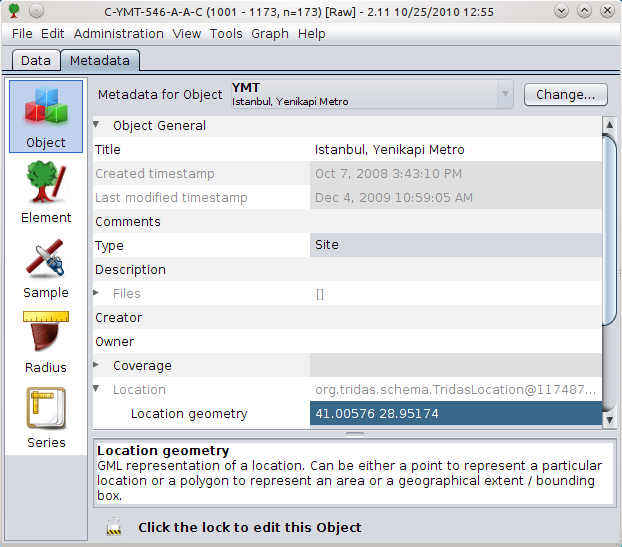
\includegraphics[width=0.6\textwidth]{Images/metadata.png}
\caption{Example of the metadata dialog.  The screen is showing the details of a TRiDaS object.  Note that the location geometry field is highlighted and so a description of what is expected in this field is given below.} 
\label{fig:metadata}
\end{figure}

When creating a new series, the metadata screens must be populated in order.  This is necessary because of the nesting of entities described above.  For instance, an element is associated with an object, so an object must be chosen because and element can be defined.  Likewise, an element must be chosen before any samples of this element can be defined.  

Much of the time the entities that you need will already be stored within the database.  Instead of re-entering data, you simply need to select the existing entry from the database, saving a great deal of time.  Depending on the situation buttons will appear at the top of the dialog to let you `choose' an entry from the database, `revert' to the previously chosen entry, `change' the existing entry to a different one from the database, or create a `new' record.

Please note that the content of these metadata screens is kept read-only by default.  To edit the values, you must first click the padlock icon to unlock the fields.  When you have finished making changes you need to press the save button to write the changes to the database before moving to another metadata screen.

Very few of the metadata fields in the TRiDaS data model are mandatory, but a few are.  In this case, these fields are highlighted with a red background.  Note that whether a field is mandatory or not can depend on the other fields that have been filled in.  For instance, the dimensions of an element are not required, but if dimensions are given then the units for these measurements must also be provided.

A number of the metadata fields are restricted with regards the values that you can enter.  These are known as `controlled vocabularies' in TRiDaS terms.  Controlled vocabulary fields are represented by drop down menus.  Similarly fields that expect numerical values (such as element dimensions) will only allow numbers.  The final method data entry method is through custom dialogs.  The only custom dialog currently implemented is for locations.  This accepts coordinates in either decimal degrees or degrees minutes and seconds.  Alternatively you can use data from a GPS handset by providing a GPS Exchange (GPX) format file containing the waypoints. The GPX format is the most common interchange format for GPS data. You can pick the relevant waypoint from the drop down menu.  You can also preview the defined coordinates on a map using the `view on map' button. 

\tip{A popular open source GPS communication tool is GPS Babel.  It is an easy to use application which can download data from the majority of GPS handsets.  See \url{http://www.gpsbabel.org} for more information.}


\section{Entering bulk metadata}
\index{Metadata!Bulk entry}
\label{txt:bulkentry}
Entering metadata on a sample-by-sample basis works perfectly well, but does not necessarily fit best with the typical workflow of a laboratory.  Samples do not typically arrive in a lab in ones and twos, rather in large quantities following a field excursion.  In this case it is most efficient to enter all the metadata for the samples as they arrive.  This is often best in terms of data accuracy as the metadata can be entered while the field notes are still fresh in the mind.

To enable the efficient entry of lots of metadata Tellervo includes the bulk data entry interface.  This can be access from the file menu and is illustrated in figure \ref{fig:bulkentry}.  There are three pages, one each for objects, elements and samples.

\begin{figure}
\centering
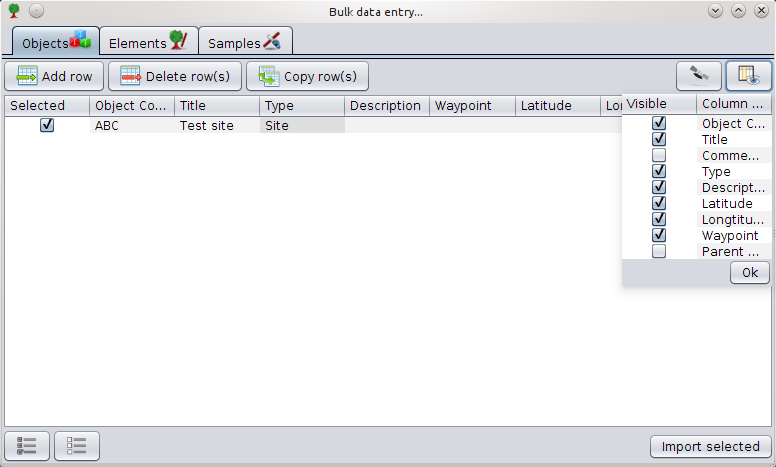
\includegraphics[width=0.6\textwidth]{Images/bulkentry.png}
\caption{The bulk metadata entry screen.  The `show/hide columns' button has been pressed showing how the user can turn on and off particular columns.} 
\label{fig:bulkentry}
\end{figure}

The interface is designed like a spreadsheet so as to be as familiar to users as possible.  Each row of the table represents a new entry in the Tellervo database.  Which columns are shown to the user is determined by the `show/hide columns' button on the top right of the screen.  

The bulk entry interface also includes support for reading GPS units.  By pressing the satellite button on the toolbar, the user can provide a GPS Exchange (GPX) format file containing the waypoint locations recorded in the field.   Tellervo will add a waypoint column to the spreadsheet with a drop down menu which will automatically populate the latitude and longitude fields for the record. 

It is common for many of the metadata fields to be same in a single field collection.  For instance, when coring trees in a forest, they are often of the same species.  Rather than requiring the user to repeatedly type the same data over and over, the `copy row' button can be used to duplicate a record, and then the user can change the few fields that are different.

When you have entered all the data you want, you can press the `Import selected' button to write the records to the database.  

\section{Metadata browser}
\index{Metadata!Browsing}
The metadata browser interface provides a convenient way to view all the metadata within your Tellervo database.  It can be accessed through the `Administration' menu.

The metadata browser contains two parts: a hierarchical representation of all TRiDaS entities in your database on the left; and a metadata viewer for the selected entry on the right.  This interface is also the best method for fixing mistakes in your database.  

Although Tellervo's database architecture maintains integrity within your data, it does come at the price of being a little more complicated to fix mislabelled series.  For instance, what if you were to measure a series 'B' and assign it to sample ABC-138-A only later to realize you misread the label and it was in fact ABC-188-A.  In a traditional file-based system, you would probably just need to rename the file you'd just created.  In Tellervo however, you need to redefine the relationship of the series within the database and reassign it to the create sample.  This is best understood when looking at the hierarchical tree in the metadata browser.  Hopefully you will see that you what you need to do is to move the series from its current position in the database to the correct one.  

The reorganization of data in this way is achieved by right clicking on items in the hierarchical tree and choosing with `merge' or `reassign'.
%% TODO - Finish


\section{Laboratory codes}
\index{Laboratory codes}
\index{Sample codes|see{Laboratory codes}}
Tellervo uses lab codes to refer to the hierarchical nature of the TRiDaS entities in the database.  The separate parts of the code a delimited by hyphens and depending on the level of the entity you are referring to, will have a different number of parts.  For instance, if you are referring to a tree (an `element' in TRiDaS terminology) then the lab code will consist of just two parts: the object code and the element code.  See figure \ref{fig:labcodes} for an illustrated example.

\begin{figure}
\centering
\includegraphics[trim = 1in 1.5in 1in 0.5in, clip, width=0.9\textwidth]{Images/TellervoSampleCodes.pdf}
\caption{Illustration of the how lab codes are built in Tellervo.  Figure courtesy of Charlotte Pearson.} 
\label{fig:labcodes}
\end{figure}

Lab codes are used throughout Tellervo to describe TRiDaS entities.  They can also be used in many places to specify entities that the user would like to choose.  For instance, in the database browser, you can type the lab code for an object, element, sample, radius or series to search the system for all the series that match the specified entity.  For instance entering `ABC-5' would search for all series associated with element `5' from object `ABC'.



\index{Metadata|)}



    \chapter{Mapping}

Corina includes an integrated open source 3D mapping system (based on NASA's award winning World Wind Java SDK) similar to the program Google Earth which you're no doubt familiar with. As mentioned in the installation chapter, this mapping system requires an OpenGL 3D capable graphics card. 

Before you can use the mapping in Corina, it must have something to map! See the chapter on Metadata (page \pageref{txt:metadata}) for information about adding coordinates to your system.

There are two ways to map data from your database. First of all, you can see a map of all the sites (i.e. TRiDaS objects) by going to Administration, then Site map. This will give you a screen like this:

\begin{figure}[hbtp]
  \caption{Screenshot showing an example of a site map.}
  \label{fig:map}
  \centering
    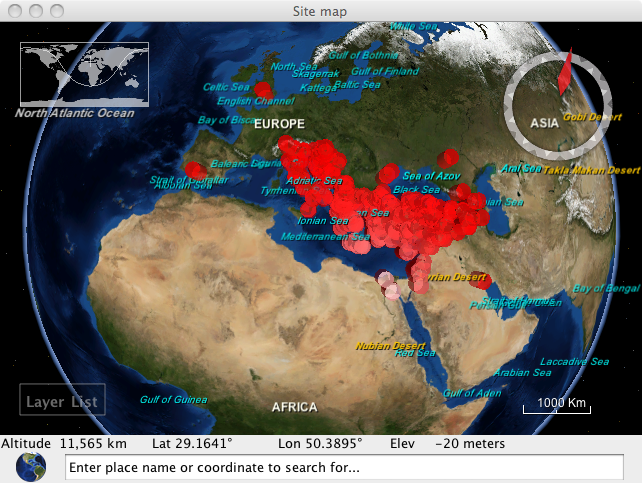
\includegraphics[width=0.8\textwidth]{Images/sitemap.png}
\end{figure}


You can also see a map of your current series if you have latitude/longitude metadata by clicking on the map tab on the main data screen. 

\section{Navigation}

You can navigate around your maps using both your mouse and keyboard.

\subsection{Mouse with scroll wheel}

\begin{description}
      \item[Pan] Left mouse button click and drag -- all directions
      \item[Zoom] Use the scroll wheel on the mouse or Left and Right mouse (both buttons) click and drag up and down
      \item[Tilt] Right mouse button click and drag -- up and down or use `Page Up' and `Page Down' on the keyboard.
      \item[Rotate] Right mouse button click and drag -- left and right Note: Crossing the top and bottom half of the screen while rotating will change direction.
      \item[Stop] Spacebar
      \item[Reset Heading] N
      \item[Reset all] R 
\end{description}


\subsection{Single button mouse}
\begin{description}
     \item[Pan] Left mouse button click and drag - all directions. L left mouse button click once to center view.
     \item[Zoom] Hold `Ctrl' on the keyboard and Left mouse button click and drag - up and down
     \item[Tilt] Hold `Shift' on the keyboard and Left mouse button click and drag - up and down or use "Page Up" and "Page Down" on the keyboard.
     \item[Rotate] Hold `Shift' on the keyboard and Left mouse button click and drag - left and right
     \item[Stop] Spacebar
     \item[Reset Heading] N
     \item[Reset all] R 
\end{description}


These controls enable you to explore your location information in 3D such as the example of Mount Vesuvius in figure \ref{fig:3dmap}.

\begin{figure}[hbtp]
  \caption{Example of 3D mapping in Corina.}
  \label{fig:3dmap}
  \centering
    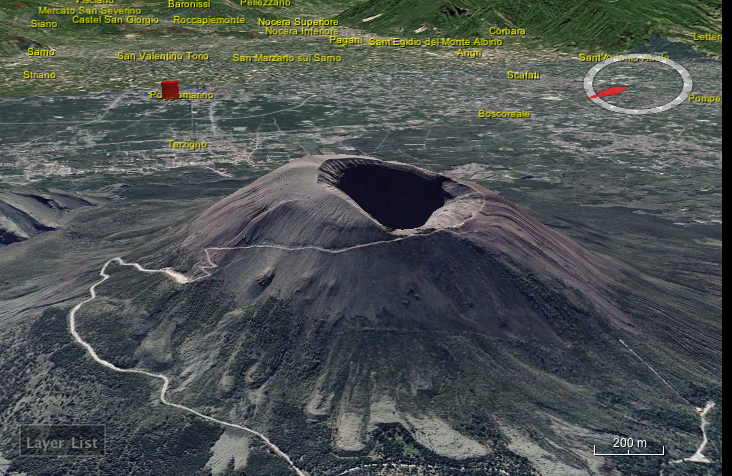
\includegraphics[width=0.8\textwidth]{Images/3dmapexample.png}
\end{figure}

Another method of navigating around the map is by using the built in gazetteer. You can enter and place name or coordinate information into the box at the bottom of the screen and you will fly to the requested location. 


\section{Interacting with data}

Each marker on the map represents either a TRiDaS object or element in your Corina database. By clicking on these pins you can get more information from the database (see figure \ref{fig:mappin}).

\begin{figure}[hbtp]
  \caption{Screenshot of a map with information pin expanded}
  \label{fig:3dmap}
  \centering
    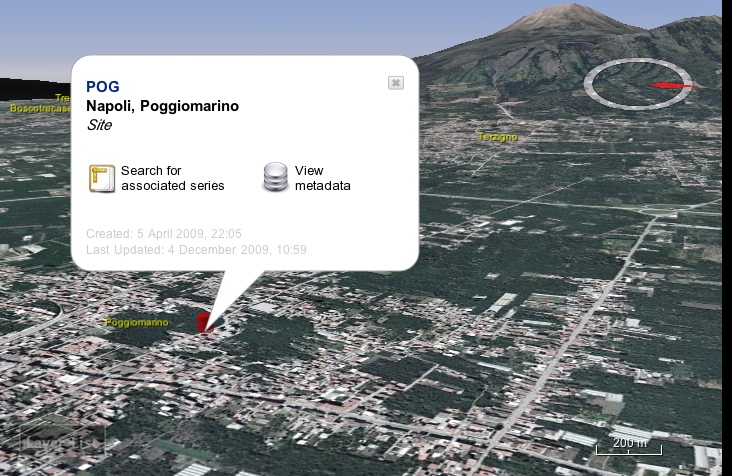
\includegraphics[width=0.8\textwidth]{Images/mappinexample.png}
\end{figure}

The example above shows the ring marker is of a site in Napoli called Poggiomarino (code name POG). You can see the option for searching for all series in the database associated with this site, and also the option for viewing all the metadata. 

\section{Background map layers}

Corina comes ready configured with basic map layers, including high resolution satellite imagery and basic political features. You can turn background layers on and off by going to View > Layers.

Map layers are downloaded on-the-fly so there is likely to be a delay when you initially visit to a new region. However, up to 2Gb of map data can be cache locally to your hard disk, so on future visits, maps should load quickly.

The mapping system in Corina includes support for remote map servers that use the OGC Web Mapping Service (WMS) standard. If you go to View > Layers > Add remote layers you will get a dialog with a tab for each WMS server configured for your system. By default this includes the NASA Earth Observation and Jet Propulsion Lab servers, but your Corina administrator can add others. By ticking layers in this list you can add data layers to your map. Your system administrator may host a map server specifically for your lab, for instance, containing high resolution plans of an archaeological site that you are working on. Figure \ref{fig:wms} shows an example overlay of sea surfaces temperatures loaded dynamically from the NASA EO server.

\begin{figure}[hbtp]
  \caption{Map screenshot with a NASA sea surface temperature overlay dynamically loaded from the NASA WMS server.}
  \label{fig:wms}
  \centering
    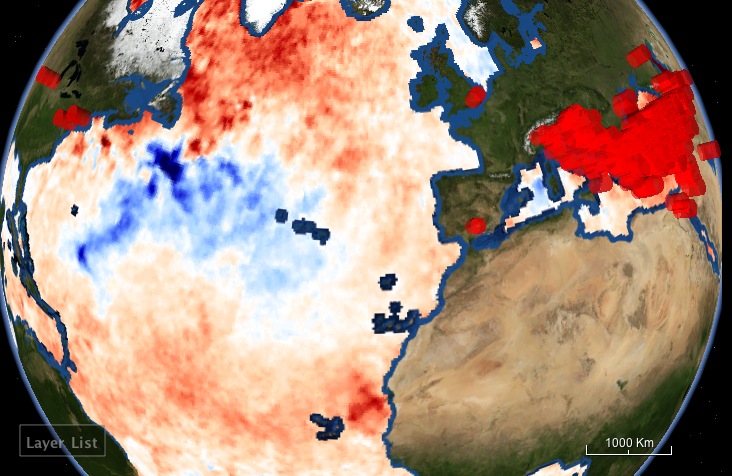
\includegraphics[width=0.8\textwidth]{Images/sst.png}
\end{figure}

\section{Data map layers}
Data map layers are controlled with the layer list in the bottom left of the screen. When viewing series, you will have the option of adding layers containing points for all the other series at the current site, and showing all the sites in the database. 


\section{Exporting maps}

You can export maps by going to File > Export map as image. For best results, maximize your map window first. You may also like to turn off various map widgets by going to the View menu. The exported image will include everything you can see on your map screen. 
    \chapter{Graphing}

The graphing component is reused in many places throughout the Corina desktop application.  The following description although based on the main graphing screen in Corina is largely applicable to all dialogs that include graphs (e.g.\ crossdating, indexing and reconciliation).  

The main method for graphing your tree-ring data is by choosing an option from the Graph menu.  Depending on the type of series you have open, the options available to you will be different.  For raw measurement series, you will just have the option to `Graph active series'.  This will give you a simple graph of the current series that you have open.  If you have a derived series open, then you may also choose `Graph component series' which will plot all the series that go to create this series, or 'Graph all series' which graphs all the component series as well as the current series.

\section{Controlling graphs}

When newly created graphs are plotted according to the scale on the axes.  A feature of Corina graphs though is that they can be manipulated directly on the screen.  Both dendrochronology was computerized, dendrochronologists would plot rings manually on to graph paper.  These paper graphs were then placed on lightboxes and moved around to enable comparisons.  The graph function in Corina emulates this behaviour allowing users to click and drag graphs around to test for visual matches.

Figure \ref{fig:graph} shows an example graph dialog.  The mouse is hovering of the blue measurement series at relative year 1040 illustrating Corina's highlighting and guide line capabilities.  A feature not shown in this screenshot is the illustration of sapwood rings.  When sapwood rings are present the corresponding years on the chart are denoted via a heavier line.

\begin{figure}[hbtp]
  \centering
    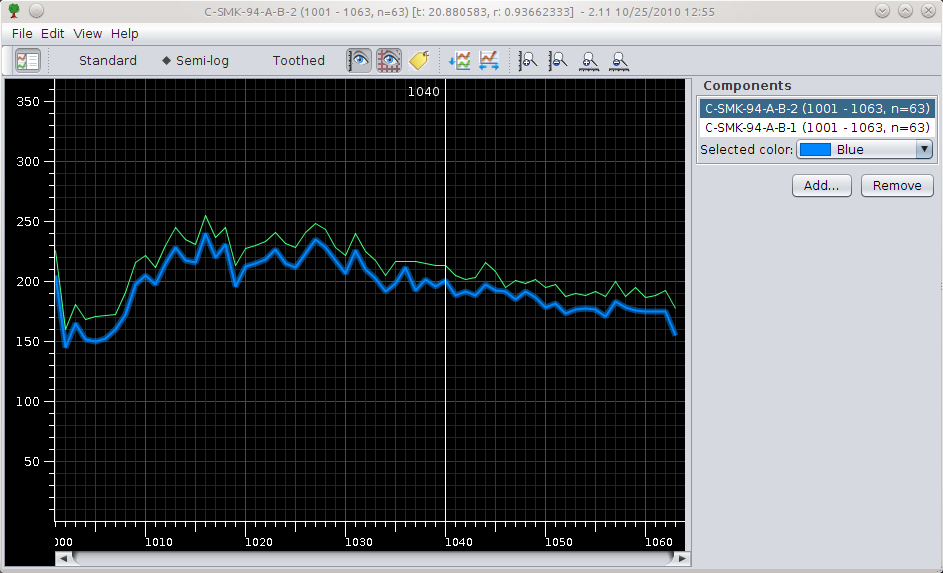
\includegraphics[width=0.6\textwidth]{Images/graph.png}
    \caption{An example graph window containing two undated series of the same sample on a semi-log graph.  Note the legend is visible with the options for adding or removing series.}
    \label{fig:graph}
\end{figure}


The layout of graphs can be changed using both the toolbar buttons and menu options.  The type of graph can be changed between a standard line graph, a semi-log graph and a toothed graph using the radio buttons.  The remaining buttons are as follows:

\begin{center}
\begin{tabular*}{0.8\textwidth}[h]{lp{10cm}}
 
\includegraphics[width=4mm]{../src/edu/cornell/dendro/corina_resources/Icons/22x22/haxiszoomin.png} & Zoom in on the horizontal axis \\
 
\includegraphics[width=4mm]{../src/edu/cornell/dendro/corina_resources/Icons/22x22/haxiszoomout.png} & Zoom out on the horizontal axis \\
 
\includegraphics[width=4mm]{../src/edu/cornell/dendro/corina_resources/Icons/22x22/vaxiszoomin.png} & Zoom in on the vertical axis \\
 
\includegraphics[width=4mm]{../src/edu/cornell/dendro/corina_resources/Icons/22x22/vaxiszoomout.png} & Zoom out on the vertical axis \\
 
\includegraphics[width=4mm]{../src/edu/cornell/dendro/corina_resources/Icons/22x22/showgrid.png} & Toggle show/hide the grid lines \\
 
\includegraphics[width=4mm]{../src/edu/cornell/dendro/corina_resources/Icons/22x22/label.png} & Toggle show/hide the series labels \\
 
\includegraphics[width=4mm]{../src/edu/cornell/dendro/corina_resources/Icons/22x22/vaxisshow.png} & Toggle show/hide the vertical axis \\
 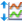
\includegraphics[width=4mm]{../src/edu/cornell/dendro/corina_resources/Icons/22x22/spreadvertically.png} & Spread the series evening up the vertical axis \\
 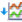
\includegraphics[width=4mm]{../src/edu/cornell/dendro/corina_resources/Icons/22x22/squeezevertically.png} & Set the baselines of all the series to zero \\
 
\includegraphics[width=4mm]{../src/edu/cornell/dendro/corina_resources/Icons/22x22/fitcharthoriz.png} & Resize graph to fit horizontally \\
 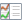
\includegraphics[width=4mm]{../src/edu/cornell/dendro/corina_resources/Icons/22x22/legend.png} & Toggle show/hide the legend\\
\end{tabular*}
\end{center}

There are also a number of keyboard shortcuts that you might find useful:

\begin{description*}
 \item[Tab] : Cycles through each graph component
 \item[Ctrl+W] : Increase vertical scale
 \item[Ctrl+S] : Decrease vertical scale
 \item[Ctrl+A] : Increase horizontal scale
 \item[Ctrl+D] : Decrease horizontal scale
 \item[Up arrow] : Moves selected graph up by 10 units
 \item[Down arrow] : Moves selected graph down by 10 units
 \item[+] : Moves selected graph up by 1 unit
 \item[-] : Moves selected graph down by 1 unit
 \item[HOME] : Scroll to first year of series
 \item[END] : Scroll to last year of series
 \item[PAGE UP] : Scroll left by one page width
 \item[PAGE DOWN] : Scroll right by one page width
 \item[SPACE] : Sets horizontal origin of all graphs to the same value 
\end{description*}

\section{Exporting graphs}

To export your graphs for use in reports you can go to \menutwo{File}{Export plot as PDF file}, or \menutwo{File}{Export plot as PNG file}.  This presents you with a dialog for setting the colors, labels and size of the exported image.  This functionality is due for an overhaul in the future to provide more flexible support for publication quality graphics.  

    \chapter{Importing and exporting}
    \chapter{Curation and Administration}
\index{Curation|(}


\section{Laboratory workflow}
\index{Workflow}
Corina includes a number of functions to assist you with the curation of your physical sample collection.  To understand how these are designed to assist users, we must first consider the workflow within a laboratory.

In research laboratories, samples generally come to the lab in large batches following field collection.   In this case the typical workflow may be as follows:

\begin{enumerate*}
 \item Collect samples and record field notes as accurately as possible
 \item On returning to the lab enter field notes as soon as possible into the `bulk data entry' interface
 \item Print sample barcode labels
 \item Prepare physical samples and label with barcodes
 \item Assign samples to storage boxes
 \item Measure samples, using barcodes to recall metadata from database
 \item Crossdate samples / build chronologies
 \item When all samples from a box are completed register box as archived and then store
\end{enumerate*}

For commercial labs offering dendrochronological dating as a service, samples more likely to arrive in smaller batches.  In this case, the bulk data entry interface may not be the most efficient method for entering metadata.  In this case the user may simply prefer to use the \menutwo{File}{New} method for each sample.  

Either way, the concept behind the curation of a collection in Corina revolves around the accurately recording as much metadata about a sample as possible, then labeling the physical sample with a label containing a barcode for Corina and sample code for the user.  By entering a sample into the database as soon as it enters the lab, it can be traced throughout the workflow.  When a chronology is built, it is easily to quickly and efficient locate all samples that have been used.  By assigning samples to boxes, groups of similar samples (e.g.\ from the same site) can also be easily stored together and located quickly and efficiently.  


\section{Barcodes}
\label{txt:barcodes}
\index{Barcodes}

Barcodes allow you to keep track of what samples you have and where they are stored.  Although it is not essential to use the barcode functions, we strongly suggest you do because they save time and money, but most importantly they greatly reduce the scope for erroneous data entry.  For instance, when measuring a sample a user simply scans its barcode and all the relevant metadata is retrieved from the database, rather than relying on them to enter data manually.  Barcodes have been routinely used in the retail industry since the 1980s.  They can be equally as useful in dendrochronology laboratories.

Corina creates and reads barcodes for samples, measurement series and boxes.  Each barcode encodes the unique identification code stored in the Corina database for each of these entities.  Due to Corina's use of universally unique identifiers (UUIDs), these codes are guaranteed to be unique opening the opportunity of labs to loan samples, much like libraries do with books.  There are many styles (or `symbologies') of barcodes in use today, but Corina uses one of the most common (Code 128) which is supported by the vast majority of barcode readers.  For a detailed discussion on the specifications of the Corina barcode see section \ref{txt:barcodeSpecs}.

Basic barcode readers are now cheap and widely available, with basic devices retailing for a few tens of dollars.  Most are characterized as `keyboard interface devices' and work like an automated keyboard, typing in a string of characters when a label is scanned.  

Within the Corina application, whenever the user is required to specify a box, sample or series, they have the option of typing the human readable lab code or scanning the barcode. By using the barcode, the user can be sure they are not entering typographic errors so we recommend using barcodes whenever possible. 

The most important barcode is the label for the physical wood sample.  These are easily generated through the \menuthree{Administration}{Labels}{Sample labels} menu entry.  Currently the layout of these labels is fixed, but in the future we aim to provide different styles.  

\subsection{Sample labels}
\index{Labels!Samples}
Before labels can be generated, metadata entries the sample level must have been made in the database.  This is typically done using the `bulk data entry' interface (see page \pageref{txt:bulkentry}).  If samples are already in the database, the user needs to select the object of interest in the label creation dialog to see all the available samples.  It is then just a matter of selecting the samples of interest and moving them into the `selected' column.  Once the list is populated (samples from multiple objects can be included), then you can either click `Preview' to see a PDF of the labels, or `Print' to print directly.

\begin{figure}[hbtp]
  \centering
    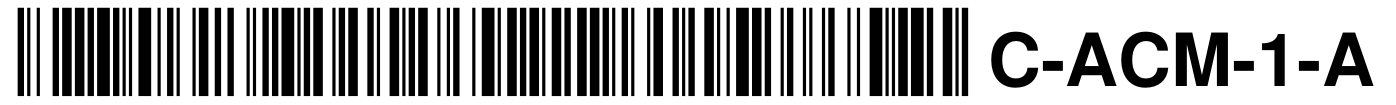
\includegraphics[width=100mm]{Images/samplebarcode.png}
    \caption{An example of a sample barcode produced by Corina for the Cornell lab.  Note the label also includes the human readable code for the sample.}
    \label{fig:graph}
\end{figure}

The current label style is designed to fit on standard core mounts and most samples.  There are no widely available die-cut labels that fulfill this need, so the labels are intended to be printed on archival grade full page sheet labels (e.g.\ Avery\textsuperscript{\textregistered} layout 6575), and then manually guillotined.  

\subsection{Box labels}
\index{Labels!Boxes}
The procedure for printing box labels is the same as for samples.  Samples must have already been assigned to boxes before the label is printed (see section \ref{txt:assignToBox} for details).  To print (or preview) box labels go to \menuthree{Administration}{Labels}{Box labels}.  The label style is designed to be printed on $5'' \times 8{1 \over 8}''$ labels, two per sheet such as the Avery\textsuperscript{\textregistered} 6579 layout.  An example is shown in figure \ref{fig:boxlabel}.

\begin{figure}[htbp]
  \centering
    \setlength\fboxsep{0pt}
    \setlength\fboxrule{0.5pt}
    \fbox{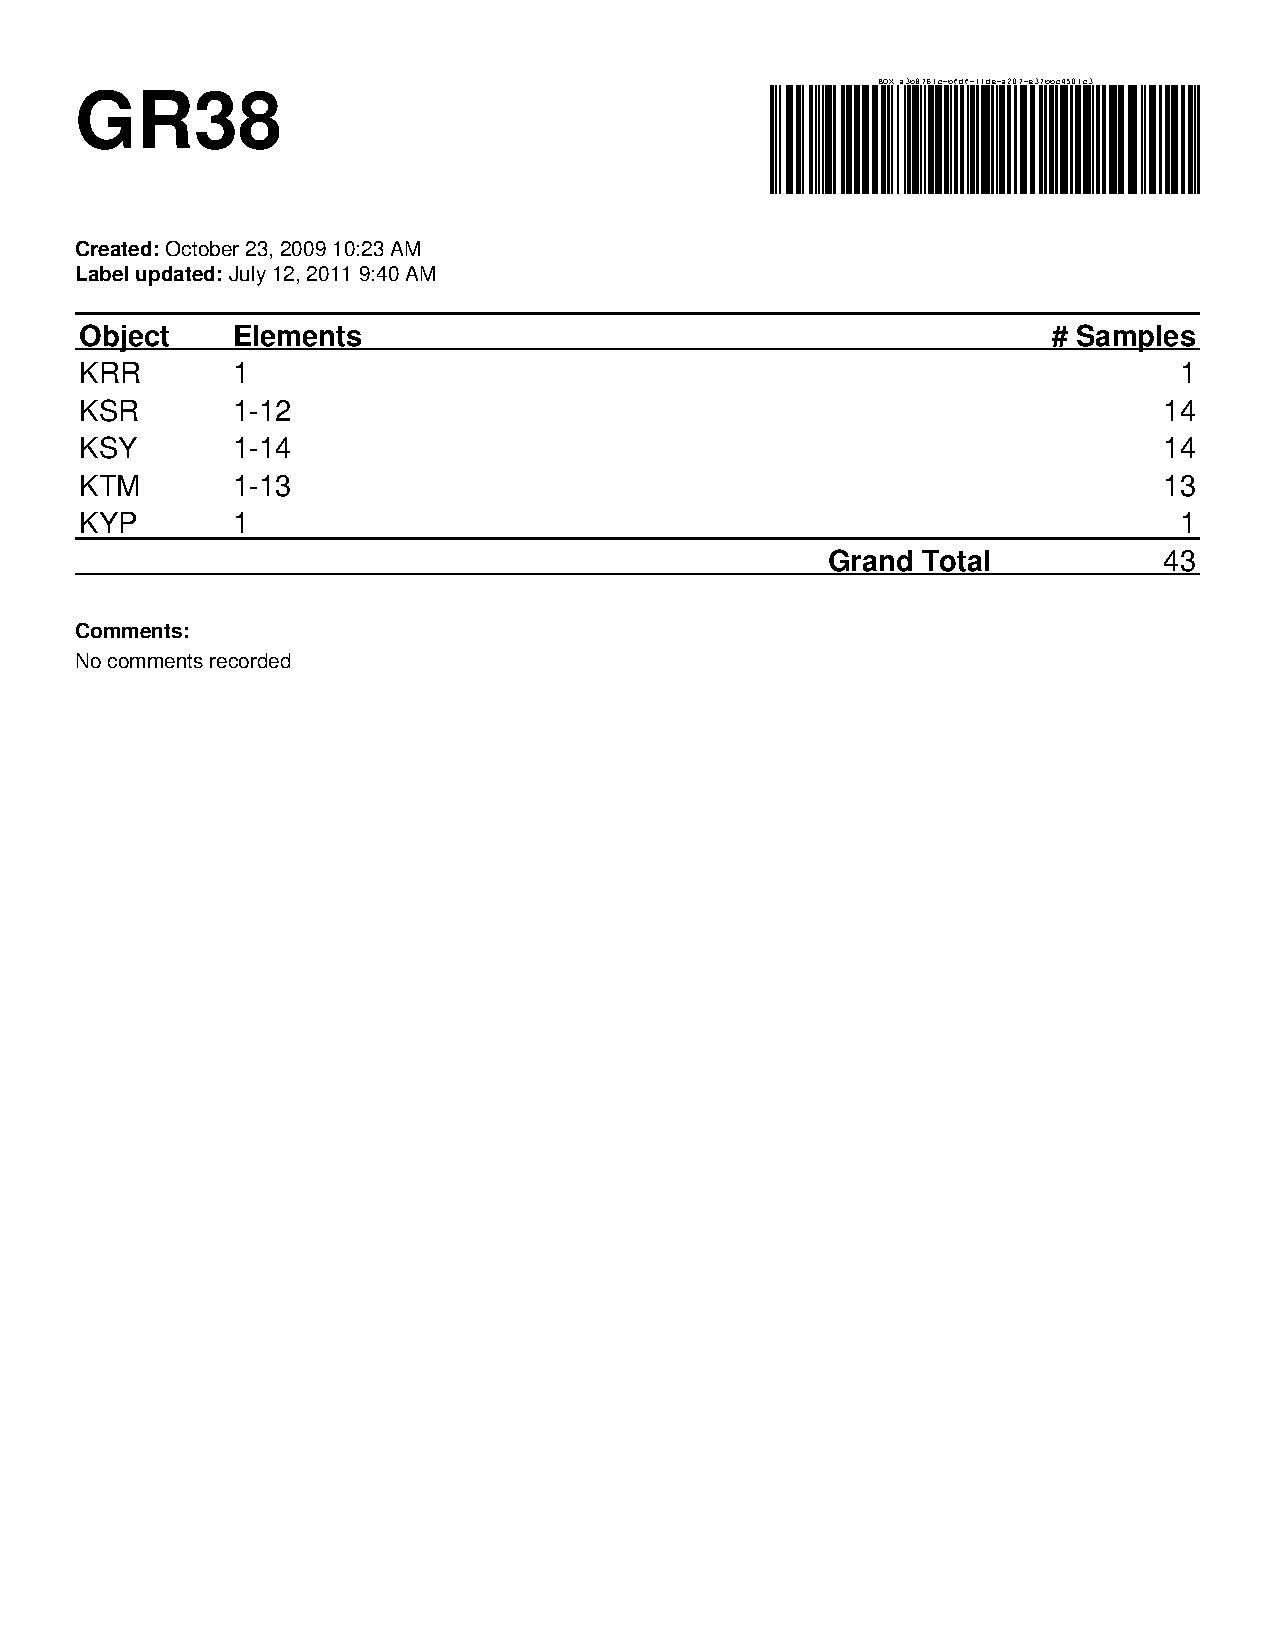
\includegraphics[width=\textwidth, trim=0 15cm 0 0]{Images/boxlabel.pdf}}
    \caption{An example of a box label from the Cornell collection. The label provides a human readable name for the box (GR38), a barcode for accessing the box details within Corina, and a summary of the samples contained within the box.}
    \label{fig:boxlabel}
\end{figure}

\info{Until dynamic label styles have been implemented, box labels will print one per page.  To make use of the second label on the page, the same sheet should be fed through the printer a second time.}

\subsection{Series barcodes}

Series barcodes are printed at the top of a standard series report (see figure \ref{fig:seriesreport}).  These are produced through the \menutwo{File}{Print}, or \menutwo{File}{Print preview}, menus.  

\begin{figure}[p]
  \centering
    \setlength\fboxsep{0pt}
    \setlength\fboxrule{0.5pt}
    \fbox{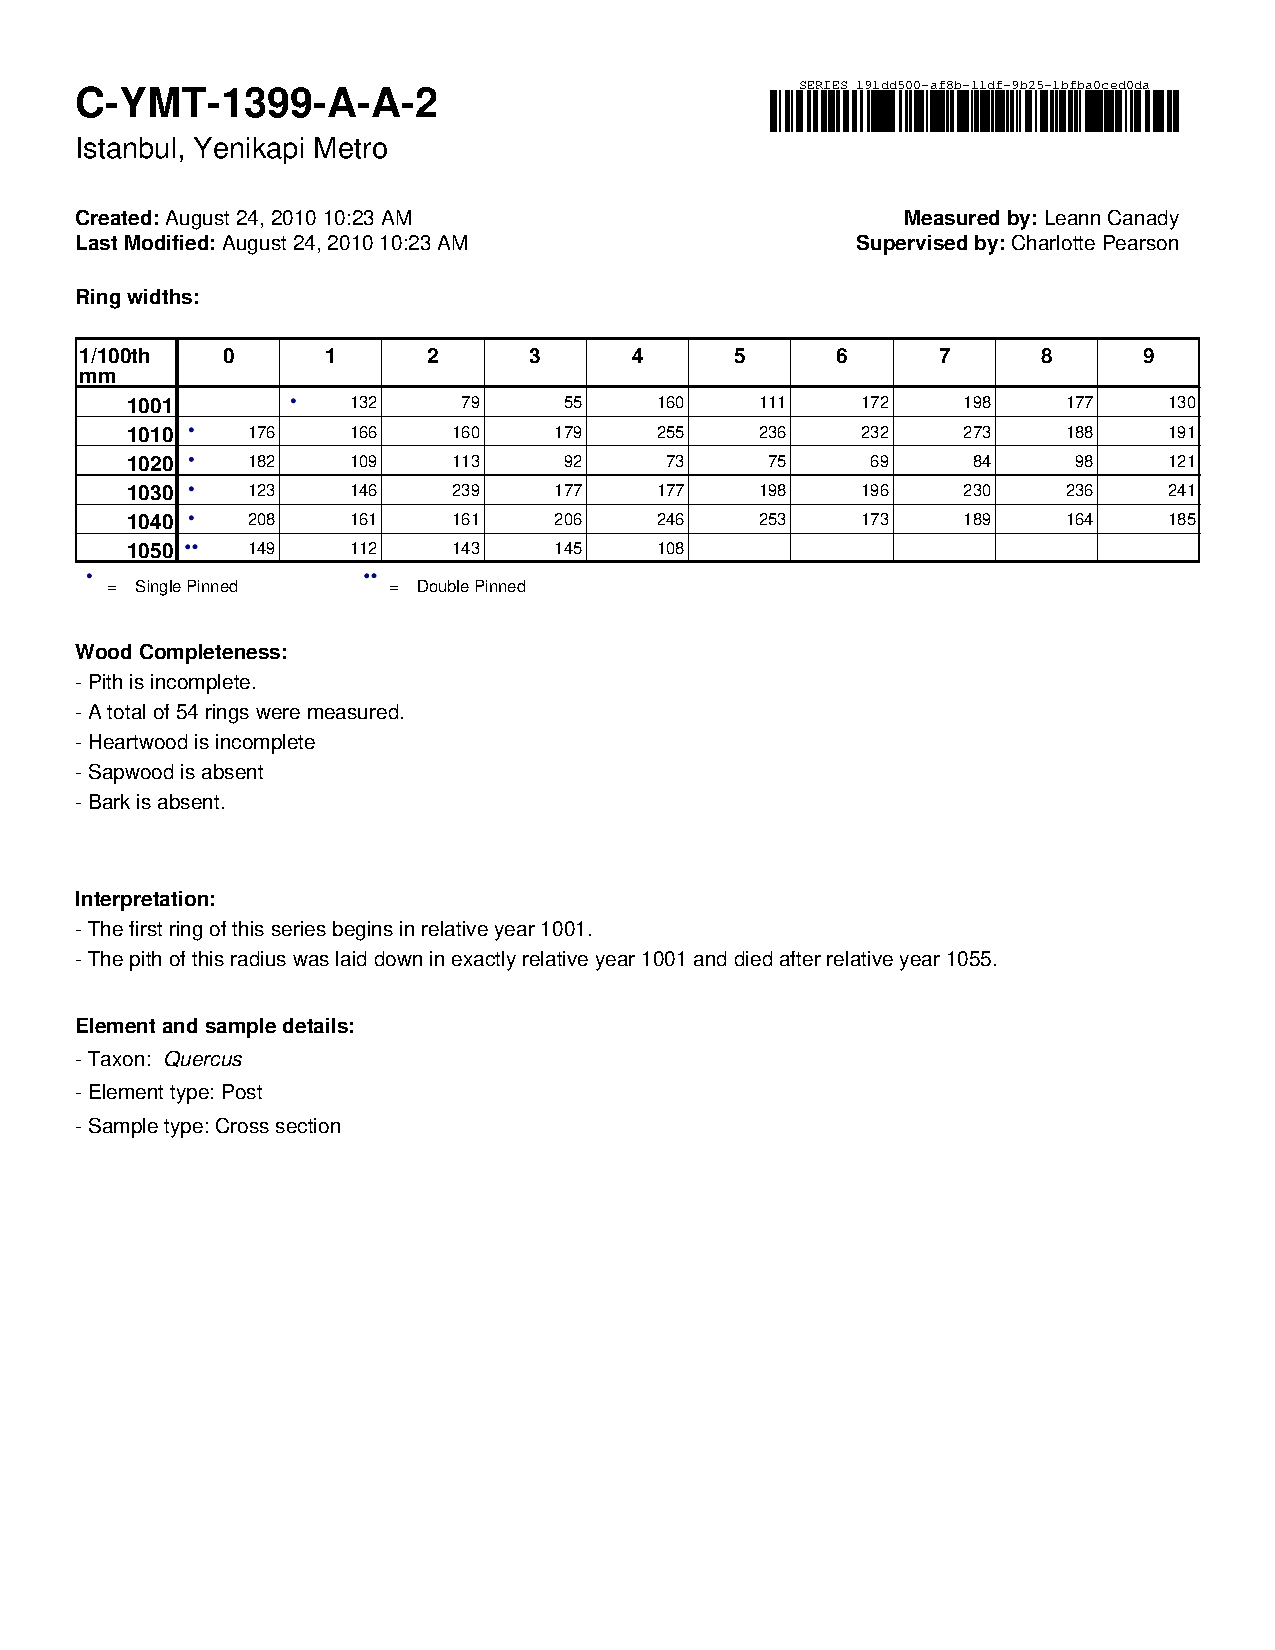
\includegraphics[width=\textwidth]{Images/seriesreport.pdf}}
    \caption{An example of a report showing barcode and basic metadata about a series.  }
    \label{fig:seriesreport}
\end{figure}


\section{Storage boxes}
\label{txt:assignToBox}
\index{Boxes}
Corina uses the term `box' to refer to the collection of samples you archive.  Many labs (including Cornell) use cardboard bankers boxes to store samples once they are completed, but the same box concept could refer to draws or shelves in your collection.

\subsection{Creating and editing boxes}
\index{Boxes!Creating}
\index{Boxes!Editing}
Records for boxes in the system are created and edited through the \menuthree{Administration}{Curation}{Box details} menu.  To editing an existing box, you can scan the barcode label on the box, or select from the list.  To create a new box, click the `Create new box' button and enter its details.  There is no restriction on what boxes should be called, but it is probably easiest if you use some sort of numerical sequence to assist with organizing the boxes in your store.  At Cornell, we use a two part name for each, the first being the year of collection, the second being a sequential number (e.g.\ 2009-11).

\index{Sample!Assign to box}The contents tab lists all the samples that have been assigned to this box.  To add new samples, simply click the `Add sample to box' button and scan the sample's barcode.  

\subsection{Inventory}
\index{Inventory}
An important feature of any collection management system is the ability to perform an inventory on the collection.  Even with the most robust system, samples will always go astray so its important to be able to periodically check that the boxes contain what you expect.

The `Contents' tab of the Box details dialog contains a feature to assist with this.  Next to the list of samples that are recorded as present, there is a temporary checklist column.  By checking the boxes for each sample actually stored in the box it is easy to see which samples have been mislaid.  If the `Mark unchecked as missing from box' button is then pressed, the date and time the discrepancy was noted is then recorded in the comments field for the box.

\subsection{Checking boxes in and out}
\index{Boxes!Checking in and out}
Corina includes function for checking boxes in and out of a store, much like when a book is borrowed from a library.  The \menuthree{Administration}{Curation}{Check out box from store} and \menuthree{Administration}{Curation}{Return box to store} menus do just this.  You can either scan the box barcode or select the box from the drop down menu.  These options record when a box is checked out/in and by whom.  These details can be seen by users in the box details dialog.

\subsection{Locating samples}
\index{Sample!Locating}
As you might expect, Corina also includes a function for locating your physical samples.  This is available in the \menuthree{Administration}{Curation}{Find a sample} menu.  There are three methods for locating a sample: via barcode; via lab code; and manually by object/element/sample.  

If you have the sample in your hand and you simply want to know which box it should be returned to you can scan the barcode.  If you are looking for a sample and you know its lab code then you can enter this instead.  Alternatively, you can use the drop down menus to search for one or more samples at once.  For instance, you can locate all the samples for a particular object and element.


\index{Curation|)}
    \chapter{Indexing}
\index{Indexing|(}

Trees tend to put on big rings when they're young, and smaller rings when they get older. Some trees put on very large rings, while others put on very small rings. These variations in growth can make it difficult to crossdate samples.  Some dendrochronologists therefore prefer to index or normalize their ring width data before combining into chronologies.

Indexing is a manipulation you can perform on your data to make it easier to crossdate.

The procedure for indexing is as follows:

\begin{enumerate*}
   \item You open a series (raw data)
   \item You ask Corina to index it
   \item Corina shows you some possible curves
   \item You pick a curve (based on its graph, statistical scores, and your expectation of how the tree is growing)
   \item Corina converts each year's ring width to a ratio of actual growth to expected growth for that year
   \item You save the series (indexed data) 
\end{enumerate*}

Indexing changes the units of a dataset. A raw sample has units of hundredths of a millimeter (0.01 mm) or microns. An indexed sample has units of parts per thousand (0.1\%, or \textperthousand).

This doesn't cause a problem with crossdating. The t-score normalizes all samples as part of its test, and the trend only cares if the values are increasing or decreasing. For more information on crossdating and chronology building, see chapter \ref{txt:crossdating}.  It does, however, cause a problem with `summing' since summing needs to take the average (what's the average of 1mm and 75\%?). Therefore, the samples in a sum must be either all raw, or all indexed. 

\section{Types of index}

There are a total of six different indexing methods available in Corina:

\subsection{Exponential Index}
\index{Indexing!Exponential}
\index{Expontential index|see{Indexing}}
This is the most commonly used index as it matches the way trees typically grow. Quickly when young and then gradually slower.  An exponential index is therefore by far the most common index you'll use as 9 times out of 10 this will be the best choice. 

This index tries to fit an equation of the following form to your data, searching for the best values of $a$, $b$ and $p$. 
\begin{itemize}
 \item $y = a + be-px$ 
\end{itemize}

\info{This is sometimes called a negative exponential index, because the exponent is negative. Corina doesn't require that the exponent is negative, but if it's not, using this index probably isn't such a good idea; it means the tree is generally getting bigger, not smaller.}

The least-squares algorithm used comes from \citet{CLR}; the matrix solving function comes from \citet{vanLoan}.

Sometimes the exponential index does a lousy job. If a tree is living in a crowded area and the trees around it get cut down, suddenly it has much better growing conditions, so it might grow faster as it gets older, instead of slower. If you tried to use an exponential curve on a tree like this, it would exaggerate this growth, and useful data would get flattened out.

The result is you're looking at the growing conditions of this one tree, so it's not going to crossdate as well.

Alternatively, imagine you are working on a tree with a fire scar that has a few very large rings. An exponential index wouldn't take much notice of this, because most of the sample is still shaped like an exponential curve, but when you applied it they would be grossly out of proportion. For these types of samples, there are other indexing algorithms available.


\subsection{Polynomial Index}
\index{Indexing!Polynomial}
\index{Polynomial index|see{Indexing}}
When you ask Corina to perform a Polynomical Index it tries to fit a polynomial curve to your data using the following equation: 

\begin{itemize}
\item $y = a_{n}x^{n} + a_{n-1}x^{n-1} + \dots + a_{2}x^{2} + a_{1x} + a_{0}$ 
\end{itemize}

You decide what degree polynomial, n, to use and Corina automatically finds the best values of $a_{0}$, $a_{1} \dots a_{n}$, to fit your data. 

\subsection{Horizontal Line Index}
\index{Indexing!Horizontal}
\index{Horizontal index|see{Indexing}}
This only changes the magnitude not shape of the curve and is used when you would link to combine raw and indexed data together.  It is a special case of polynomial where the horizontal line is equal to the average value. 

\begin{itemize}
\item $y = x_{avg}$
\end{itemize}

This index is not used for crossdataing because dividing each value by the same value doesn't change the shape of the curve, only its magnitude. A horizontal line index is, however, useful because every element in a sum must use the same units, either raw or indexed. Therefore if you want to include a raw sample with an indexed sample then a horizontal line index can be used to convert the raw sample without otherwise altering the shape of the curve. 

\subsection{Floating Index}
\index{Indexing!Floating}
\index{Floating index|see{Indexing}}
This is a running average of the 11 surrounding years. The adaptive index is generally used as a ``last resort'' when both exponential and a high-degree polynomial have failed. It is simply the average of the eleven surrounding years:

\begin{itemize}
\item $ind_{i} = 1/11 (data-{i-5} + data_{i-4} + \dots + data_{i+4} + data_{i+5}$ 
\end{itemize}

This index was originally called floating average, probably in reference to the fact that the index curve ``floats'' around, not following any explicit $y=f(x)$-type formula. But people tended to call it floating, and then floating-point, which means something very different. You might still hear people calling this index by these other names.

\subsection{High-Pass Filter Index}
\index{Indexing!High-pass filter}
\index{High-pass filter|see{Indexing}}
The high-pass index is a more general case of the adaptive index. Instead of simply taking the average of 11 values, it takes a weighted average. It's an example of a ``high-pass'' filter because high-frequency signals can pass through, but low-frequency signals are filtered out.

The default is ``1-2-4-2-1'', meaning:

\begin{itemize}
\item $ind_{i} = 1/10 (data_{i-2} + 2{\cdotp}data_{i-1} + 4{\cdotp}data_{i} +2{\cdotp}data_{i+1} + data_{i+2})$ 
\end{itemize}

This comes from \citet{Cook81} who used it as a discrete filter before moving to a cubic spline. Note that almost half ($4/10$) of the computed value is simply its old value. The high-pass index is nearly the same as the input, so the $\chi^2$ values are usually the lowest, therefore do not choose this index solely on a low $\chi^2$ value. 

\subsection{Cubic Spline Index}
\index{Indexing!Cublic spline}
\index{Cublic spline|see{Indexing}}
Cubic splines are a very specific type of high-pass filter. A cubic spline curve is created by combining a collection of cubic (3rd degree polynomial) functions.

There are many methods for constructing cubic splines through a dataset. The algorithm used by Corina has a parameter, s, which controls how tightly the spline fits the data. A lower value fits the data more tightly, a higher value fits the data more loosely. Therefore, s=0 fits the data exactly while s=1 is a simple line. A good starting point for dendro data seems to be around $s=1x1016$.

Cubic splines were first used for dendro by \citet{Cook81} using an algorithm from \citet{Reinsch67}.

You can change the s-value used for the subic spline in the preferences. You might use a cubic spline in the same cases you would use a high-pass filter e.g.\ when the sample doesn't generally follow an exponential or polynomial curve very well, perhaps due to a fire scar. 

\section{Indexing data}
\index{Indexing|textbf}
To index your data, first you need to open the series you would like to index.  Next choose \menutwo{Tools}{Index} to display the indexing dialog (figure \ref{fig:index}).

\begin{figure}[hbtp]
  \centering
    
\includegraphics[width=0.97\textwidth]{Images/index.png}
    \caption{Indexing dialog showing the original data in blue, the exponential index of this data in green, and the normalized data in red. }
    \label{fig:index}
\end{figure}

From the indexing dialog you can then choose which type of index to apply to your data.  The table on the right show the available options along with the $\chi^2$ and p values to help you choose the correct index to use. The graph shows your original data, the index line and the result of applying the index to the data and changes dynamically as you pick between different indexing methods. Once you have decided which index you want to use, select it, and click OK ensuring that you have given your data series a new version number.

\index{Indexing|)}
    \chapter{Crossdating and chronology building}
\label{txt:crossdating}
\index{Crossdating|(}

All algorithms work in pretty much the same way. There's a ``fixed'' sample, and there's a ``moving'' sample. Imagine you have printouts of their graphs on translucent paper. The fixed graph is taped to a table, and you can slide the moving sample left and right. This is actually how it was originally done, on graph paper, with one inch per decade. Start with the moving sample to the left of the fixed sample, overlapping it by 10 years. Look at how well the graphs match: this is the first score that's computed. Slide the moving sample to the right one year and so on until you reach the end.

You could do it all simply by moving graphs and eyeballing the crossdates like this but there are hundreds of sites and millennia of chronologies you'll want to crossdate your samples against, so that would take a while. Corina has a few algorithms to find likely crossdates almost instantaneously. They aren't perfect, though, and all crossdates should be inspected visually to ensure they are a good fit. 

\section{Algorithms}
Corina includes a total of five different algorithms for crossdating:


\subsection{T-Score}
\index{Crossdating!T-Score}
\index{T-Score}
The t-score is the classic crossdate. Everybody quotes t-scores: if you want to brag about how good a cross is, you tell them your t-score. Unfortunately, every dendro program seems to have a slightly different implementation of tscore, so the numbers you get from Corina might not be exactly comparable to the numbers from other programs. 

The version Corina uses is based on the algorithms given in \citet{Baillie73}, though with some apparent bugs corrected. In the following equations, $x_{0}, x_{1}, x_{2}, \dots$ are the data of the fixed sample in the overlap, $y_{0}, y_{1}, y_{2}, \dots$ are the data of the moving sample in the overlap, and N is the length of the overlap.

The first step is to make each dataset bivariate normal by replacing each value with the mean of the values around it, and then taking its natural logarithm.  The preparation for the T-Score is therefore done as follows and is done to both the fixed and moving series:

\begin{itemize}
 \item $x_{i} \leftarrow {x_{i-2} + x_{i} + x_{i+1} + x_{i+2} \over 5}$
 \item $x_{i} \leftarrow ln(_{xi})$
\end{itemize}

The student's T computation is then done as follows:

\begin{itemize}
 \item $s_{xy} = \Sigma x_{i} y_{i} - N (x_{i} - x_{avg}) (y_{i} - y_{avg})$
 \item $s_{xx} = \Sigma x_{i}^{2} - N (x_{i} - x_{avg})^{2}$
 \item $s_{yy} = \Sigma y_{i}^{2} - N (y_{i} - y_{avg})^{2}$
 \item $r = {s_{xy} \over \sqrt{(s_{xx} s_{yy})}}$
 \item $t = r \sqrt{{N-2\over 1-r^{2}}}$
\end{itemize}

The t-score is called a ``parametric'' algorithm, because it takes into account the magnitudes of the samples.

A t-score is considered statistically significant if it's greater than a certain value. Just what this value is varies with the length of the overlap between the samples: a 500 year overlap can have a t-score of 2.6 and pass, but an overlap of only 15 years would have to be higher, like 3.0.  In reality most dendrochronologists require t-scores to be much higher than this, and would also insist on overlaps of many decades.


\subsection{Trend}
\index{Crossdating!Trend}
\index{Trend}
Trend is another popular crossdate statistic.  It computes the percentage of years with the same trend (going-up- or going-down-ness). Scores greater than 60\%-70\% are good. Trend is also referred to as ufigkeitsko-Gleichläeffizient, Gleichläufigkeit and Eckstein's W.

The trend is the simplest crossdate. For each sample, it computes the trend of each 2-year interval (1001-1002, 1002-1003, and so on). The trend of a 2-year interval is simply whether the next ring is larger, smaller, or the same. The trend score is the percentage of intervals in the overlap which are the same. For example, a 75\% trend (a very good score, by the way) means that for 75\% of the intervals in the overlap, both samples went up in the same years and down in the same years.

If one sample stays the same, and the other increases or decreases, Corina considers that to be halfway between a same-trend and different-trend, and gives it half a point. Trend is a ``non-parametric'' algorithm, because it only takes into account if a given ring is bigger or smaller than the previous one, not by how much. To the trend, a drop of ``100 1'' looks exactly the same as a drop of ``100 99''. Two completely random samples will have a trend of 50\%, on average. So you'd expect a trend must be greater than 50\% to be significant.

According to \citet{Huber70}, a trend is significant if:

\begin{enumerate}
  \item \textbf{$tr > 50\% + {50 \over \sqrt{N}}$} - For example a pair of samples with a 50-year overlap needs a $50+50\sqrt{50} = 57.1\%$ trend to be significant, but at a 400-year overlap need only a $50 + 50\sqrt{400} = 52.5\%$ trend. In practice, however, this doesn't tend to work terribly well. Using this scheme, there are typically about three times as many ``significant'' trend scores as t-scores, and users want this narrowed down a bit more. So take $\sigma=3$ and use:
  \item $tr > 50\% + {50\sigma \over \sqrt{N}}$ - This gives about the same number of significant trend scores as t-scores. 

\end{enumerate}

Trends are also used in reconciliation. After they've been reconciled, both readings of a sample should have 100\% trend. 

\subsection{Weiserjahre}
\index{Crossdating!Weiserjahre}
\index{Weiserjahre}
The Weiserjahre algorithm is used for crossdating summed samples (chronologies) against single samples. All of the algorithms that have been mentioned so far only compare the ring widths. This works fine for raw samples, but when crossdating summed samples, there's a lot more information available, namely, the Weiserjahre data. Wouldn't it make sense to count a [20] $19\times1$ ring more heavily than a [1] $1\div0$ ring? 19 out of 20 samples think it's an increasing year, not just 1. 

This is what the Weiserjahre cross does: for each possible overlap, it starts by counting the number of significant intervals of the master for that overlap. A significant interval is one with at least 3 samples, where at least 75\% of them have the same trend. Then it computes the percent agreement (like the trend) between the master and the raw sample for only those significant years of the overlap. Of course, for the trend of the master, it doesn't use the trend of the master; it uses the trend of the majority of its elements. They're usually the same, but not necessarily.

Another way to think about the Weiserjahre crossdate is: it's like a trend, but ignoring years where the sum has only 1 or 2 samples, or where there isn't an overwhelming trend in the sum. Also like the trend, the results are given as a percentage.


\subsection{R-Value}
\index{Crossdating!R-Value}
\index{R-Value}
The R-value, or correlation coefficient, is a crossdate which you'll almost never use. It's not terribly useful to dendrochronologists, but statisticians might want to know its value, so Corina makes it available.

The R-value is used in the T-Score, the T-score being defined in terms of the r-value and the overlap, N. If you look at the equations for calculating a T-Score you will see on the penultimate line: 

\begin{itemize*}
 \item $r = {s_{xy} \over \sqrt{(s_{xx} s_{yy})}}$
\end{itemize*}

An r-value can range from 0.0 (no correlation) to 1.0 (perfect correlation). 
 
\subsection{D-Score}
\index{Crossdating!D-Score}
\index{D-Score}

The D-score (AXE), is a combination of the T-Score and Trend.

\begin{itemize*}
 \item $D = (tr - 50\%) \times t $
\end{itemize*}

Corina considers 40 to be the threshold for significant AXE. 

\section{Crossdating series}
\index{Crossdating!Performing}

\section{Managing chronologies}
\index{Crossdating!Managing chronologies}
\index{Chronologies}

\index{Crossdating|)}

    
\chapter{The Tellervo server}
\label{txt:servermaintenance}

For basic day-to-day running of the Tellervo server, you simply need to make sure that the server is running.  All other interaction and managment (creating users, granting permissions, accessing data) is done through the Tellervo desktop application.  This section, however, outlines a number of aspects of the server that advanced users may find useful.

\section{Backing up and restoring your database}
\index{Server!Backup}
\index{Backup}
As with any computer system it is important for you to back regular backups of your data to guard against hardware (as well as human!) errors. The two main methods for doing this are outlined below:

\subsection{Backup whole Virtual Appliance}
\label{txt:BackupVA}
The simplest method is to make a copy of your entire Virtual Appliance, but this does have a number of drawbacks.  The first is that you need to shut down your server before you can make the backup so this is only possible if server `downtime' is not a problem for your lab.  The second drawback is that it makes a copy of your entire server including the whole operating system, therefore each backup takes a lot more space.  

\begin{enumerate*}
 \item Open VirtualBox
 \item If you server is running you will need to do a full shutdown.  From the server console type \verb|sudo halt| then once it has halted you can close the console window and select `Power off the machine'. 
 \item Select your virtual machine in the list on the left and go to \menutwo{File}{Export Appliance}.
 \item Follow the wizard, specifying a file where you'd like to back the server up to.  Keep in mind that this will contain a complete copy of the server (including operating system) so could be 1Gb or more.
\end{enumerate*}

\subsection{Restoring a Virtual Appliance backup}
If you have followed the instructions in section \ref{txt:BackupVA} to backup your Virtual Appliance the steps to restoring your server are very similar to how your initially installed it.  Simply open VirtualBox, then go to \menutwo{File}{Import Appliance} and select the backup file that you made.  Follow the wizard and it should restore your server.  You can restore onto the same computer that was originally running the virtual machine (remember to give it a new name though if this is the case) or alternatively to any other computer with VirtualBox installed.  This method can therefore be used to share entire databases.


\subsection{Backup PostgreSQL database}
The more standard way of backing up your database is to do a dump of the PostgreSQL database itself into a large text file.  This is a little more involved, so it is only recommended if you are familiar with command line and/or Linux.  You can create the file with a command like the one below, but you should read up on pg\_dump so that you understand the possible options that you can use.

\code{pg\_dump -Fc -f /folder/and/file/to/make/mybackup.sql database\_name}

For example the following line will backup the database called `tellervo' (the standard name for your database) into a file called backup.sql in the tmp folder.  Keep in mind that the tmp folder is cleaned each time the server is booted.

\code{pg\_dump -Fc -f /tmp/backup.sql tellervo}

It then makes sense to transfer this backup off the virtual machine onto a separate computer as per normal backup procedures.  If you are familiar with Linux you could do this by using SFTP or similar transfer protocols.  If you just want a quick and dirty method, you could save the backup.sql file to /var/www/tellervo-server/ and then you can access the file from any web browser at the address http://your.server.ip/tellervo-server/backup.sql.  Keep in mind though that anyone could potential download the file as long as it is left there so you will want to delete it as soon as you have transferred it.  You can do this from the server command line by typing sudo rm /var/www/tellervo.org/backup.sql.  


\subsection{Restoring a PostgreSQL database}
To restore your database from a backup file you can use the standard PostgreSQL command line tool psql to populate an empty database:

\code{createdb tellervo\_new}
\code{psql tellervo\_new < /tmp/backup.sql}



\section{Upgrading the server}
Upgrading the server requires you to type a few commands into the Linux command line.  First of all please ensure that you back up your Virtual Appliance and/or database before continuing.  We will always endeavour to make sure that nothing happens to your database, even if the upgrade fails for some reason (in which case the system should roll back to your previous version again), but things don't always go to plan.

\begin{enumerate}
 \item Log in to your Tellervo server console 
 \item Type the following commands: 
       \code{cd /tmp} 
       \code{wget http://url.of.new.server.file} 
       \code{dpkg --install tellervo-server-X.X.X.deb}
\end{enumerate}

The URL of the new file can be obtained from the Tellervo website.  

It would be possible for us to set up an mechanism which server administrators could opt-in to to upgrade Tellervo servers automatically.  We may deploy this in the future, but we'd rather keep the process of upgrading as a conscious decision for the foreseeable future, but especially until we are confident that the upgrade process will not compromise your database.


\section{Graphical Interface to the Virtual Appliance}
\index{Server!Graphical interface}
For those of you that are unfamiliar with Linux, the basic command line prompt is not likely to be very comfortable.  If you are interesting in looking at the server in more detail you may therefore prefer to install a full graphical interface.  Unlike Windows, there are a number of different graphical interfaces (or desktops) to choose from in Linux, the most popular being Gnome and KDE.  To install one of these you need to type one of the commands listed below.  The first line installs Gnome and the second KDE. Windows users that are new to Linux may find KDE more familiar, but Apple users may be more at home with Gnome.

 \code{sudo apt-get install ubuntu-desktop}
 \code{sudo apt-get install kubuntu-desktop}

\section{Security}
\index{Security}
The basic installation of the Tellervo server includes the standard configuration for Apache, PHP and PostgreSQL.  Although these products are considered secure by default, there are a number of measures that can be taken to make them more so.  If your server is only accessible within your local intranet (e.g. behind a robust firewall) then you may not feel it necessary to modify the standard setup.  Precautions may be deemed more important if you server is accessible from the internet.  In this case it would be wise to contact your local network administrator for further information.

\subsection{Usernames and passwords}
\label{txt:passwords}
\index{Passwords}
There are a number of default usernames and passwords setup on your server.  If your server is accessible for the internet we strongly advise you to change these defaults and anyone with knowledge of the Tellervo server could access and compromise your machine.

\begin{description*}
 \item[System user] - these are the credentials you use to log in to the command prompt in your Tellervo Virtual Appliance.  By default the user is `tellervo' and the password is `dendrochronology'.  To change this log in to the command prompt and type \verb|passwd| and follow the instructions.  There is no easy way to recover this password if you loose it.
 \item[PostgreSQL database user] - these are the credentials used by the webservice to read and write to the database and are set by the database administrator during the initial configuration of the Tellervo server. You are only ever likely to need this again if you want to directly access the database from a third party tool like PGAdminIII.  You can reset this password from the Tellervo Virtual Appliance command prompt by typing \verb|tellervo-server --reconfigure|
 \item[Tellervo admin user] - these are the admin credentials that you use to log in with in your Tellervo desktop application.  Be default the user is `admin' and the password is `qu3rcu5'.  You should change these the first time you open the Tellervo desktop application by going to \menutwo{Admin}{Change password}.
\end{description*}

\subsection{Authentication and encryption}
\index{Authentication}\index{Encryption}
Tellervo uses a relatively sophisticated method to ensure that unauthorised users cannot access the Tellervo database through the webservice.  It is loosely based around http digest authentication and uses a challenge and response scheme.  This makes use of cryptographic hashes (a relatively short digital fingerprint of some data but which cannot be decompiled to retrieve the original data) and nonces (a pseudo-random string used just once). All hashes used in the Tellervo webservice use the MD5 algorithm. This decision will be periodically reviewed to ensure that MD5 is the most appropriate and secure algorithm to use. Whilst an MD5 hash of a short phrase can be compromised, the length and randomness of the original data means with current cracking techniques this is essentially impossible.   For a complete description of Tellervo's authentication procedure see section \ref{txt:authentication}.

The default Tellervo server setup, however, uses standard HTTP protocol to communicate between the server and the desktop application.  This is the same protocol used for the majority of web pages on the internet and a determined hacker could eavesdrop on this communication.  Depending on how important and private you perceive your data you may choose to use Secure Socket Layer (SSL) to encrypt this communication.  This is the same technology used by websites such as online banking.  To make full use of this upgrade in security you will however also require a SSL certificate from an official licensing authority.  These certificates typically cost several hundred dollars per year. 


% TODO Describe how to enable SSL

\section{Directly accessing the database}
\index{Database}
\index{PostgreSQL}
Although the Tellervo database is designed to only be accessed by the Tellervo desktop application via the Tellervo server's webservice, you may decide that you'd like to directly access the database yourself.  For instance, you may like to write complicated SQL queries to probe your database in ways not currently supported by the Tellervo desktop client. 

\warn{Any changes made to the database may have drastic consequences.  We strongly recommend that you never write changes directly to the database as this can cause loss of data and corrupt future upgrades to Tellervo.}

\subsection{PGAdminIII}
\index{PGAdminIII}
One of the easiest ways to access the PostgreSQL database is through the application PGAdminIII.  This is a cross-platform open source application for communicating with PostgreSQL databases.  You can install PGAdminIII on your desktop computer and access the remotely running database using your database user credentials.  

For security reasons by default the Tellervo database cannot be accessed from computers outside of the Tellervo server.  The may sound peculiar because the webservice can be accessed from computers anywhere on the web, but the database is actually accessed by the webservice, which is essentially a user running on the same computer as the database.  To access the database \emph{directly} from a remote computer you must therefore open access first.  This is done by adding an entry to the file `/etc/postgresql/9.1/main/pg\_hba.conf'.  My personal command line text editor of choice is vim, but it is a little confusing to the uninitiated.  If you are unfamiliar with command line text editing you are probably best to use pico:

\code{sudo pico /etc/postgresql/9.1/main/pg\_hba.conf}

Scroll down passed all the comments, to the bottom of the file.  Add the following line:

%%TODO Check this is the best to suggest
\code{host  all  all   IPADDRESS/32       md5}

Make sure you replace IPADDRESS with the IP address of the computer you are trying to connect \emph{from}. This is just one style of pg\_hba.conf entry.  There are many others which allow you to restrict to specific users, computers, networks etc.  See the online PostgreSQL documentation for more details.  Save your changes and exit by doing CTRL+X.  

Next you need to make sure the PostgreSQL server is listening to requests from other IP addresses.  To do this you need to edit the postgresql.conf file like this:

\code{sudo pico /etc/postgresql/9.1/main/postgresql.conf}

making the following changes:

\begin{description}
 \item[Old line] - \verb|#listen_addresses = 'localhost'|
 \item[New line] - \verb|listen_addresses = '*'|
\end{description}

Make sure you remove the hash character at the beginning of the line.  Save the file and finally restart the Tellervo server:

\code{sudo tellervo-server --restart}

You should now be able to access your database through PGAdminIII. To do this open the application and go to \menutwo{File}{Add server}.  Specify your server's IP address is the host field, and your database username and password.


\subsection{ODBC}
\index{ODBC}
It is also possible to connect to your Tellervo database via an ODBC connection.  This allows limited access to the database from a variety of database applications including programs like Microsoft Access for which further details are given here.   To use ODBC you will need to install the PostgreSQL ODBC driver (\url{http://www.postgresql.org/ftp/odbc/}) on your desktop computer.

Once you've installed the driver you can then open a blank database in Access and go to Files, Get external data then Link tables.  In the file dialog box change the file type to ODBC Databases().  Next, select the PostgreSQL Unicode driver, then fill out the server details.  You should then be able to open the tables and views from the Tellervo server database directly from within Access as if they were local tables.  Be warned though that Access and ODBC have many limitations compared to PostgreSQL, especially with regards data types.  For this reason we \emph{strongly} recommend using this for read only purposes.  Using the ODBC connection to write changes to your PostgreSQL database is quite likely to cause serious issues. 

\subsection{PSQL}
\index{PSQL}
The final, and most advanced method is to use the psql client on your server.  This is a command line client which can be used to interrogate the database.  If you're not already familiar with psql it is unlikely that this is a good method for you to use!


\section{Tellervo server configuration}
\label{txt:serverConfig}
\subsection{Standard server configuration}
\index{config.php}
The Tellervo server can be configured using the command line tool that is installed on both the Virtual Appliance and native server installs.  It is the same tool that is run at the end of the native server install, but can be run at any time to reconfigure or test your system.  It must be run with superuser privileges therefore \verb|sudo| is required before the command.  For instance to get help on usage type:

\code{sudo tellervo-server --help}

\begin{wrapfigure}{r}{0.5\textwidth}
  \begin{center}
    \includegraphics[width=0.48\textwidth]{Images/tellervo-server-terminal.png}
  \end{center}
  \caption{Example of the output from the tellervo-server test.}
  \label{fig:serverTerminal}
\end{wrapfigure}

Possible options to pass the server are:

\begin{itemize*}
 \item `\verb|--help|' -- Display a list of the possible options
 \item `\verb|--version|' -- Display the version of the Tellervo server webservice and database currently installed
 \item \verb|`--test'| -- Run tests on the current configuration
 \item \verb|`--configure'| -- Configure the Tellervo server from scratch.  
 \item \verb|`--reconfigure'| -- Reconfigure the Tellervo server.  This should be done if the database name or user credentials change, or if the IP address of the machine is altered.
 \item \verb|`--start'| -- Start the Tellervo server
 \item \verb|`--stop'| -- Stop the Tellervo server
 \item \verb|`--restart'| -- Restart the Tellervo server
\end{itemize*} 

Figure \ref{fig:serverTerminal} shows an example of asking the server to test the configuration, with all tests passed successfully.

The command line tool stores the majority of settings in the config.php file stored in the base directory of your Tellervo webservice.  In theory you could make changes direct to this file, but we do not recommend this unless you know exactly what you're doing.


\subsection{Advanced server configuration}
\index{systemconfig.php}

In addition to the standard configuration options offered on the command line there are a number of other options that can be set.  These are not accessible via the command line because as a rule they should only be altered the Tellervo developers.  They are primarily for use by the developers as an alternative to hard coding values within the server files.  For instance, one such value is the TRiDaS version being used by the server.  This value will only ever need to be changed alongside other substantial changes to the code.  




\section{Managing map services}
\label{txt:managingmaps}
\index{Web Map Service (WMS)}
\index{Mapping!Adding layers|see{Web Map Service(WMS)}}

There is currently no interface in Tellervo that lets you specify the WMS mapping services that should automatically be available to your Tellervo users.  Each user can add servers temporarily (see section \ref{txt:userAddWMS}) but these will disappear at the end of each session.  

    \chapter{Help and support}


\section{Getting help}

At the moment your options for getting help are largely limited to contacting Peter Brewer!  Once the userbase of Corina expands we will set up forums and mailing lists to assist.


\section{Support for future development}
Both Corina Desktop and Server are free software available under the General Public License v3 (see appendix \ref{txt:licenseStart}).  This means you are free to use Corina in both academic and commercial environments.  However, when we talk about `free software' (as the license explains) we are talking about freedom of use, not free as in price.  Corina has inevitably cost a great deal to develop over the years and while you are not asking for a direct contribution, we do need your support for future development.

If there is particular functionality that you would like to see implemented in Corina, under the open-source model this can be done in a number of ways:

\begin{description}
 \item[Implement the feature yourself!] -- If you are able to program in Java then we would be delighted to assist you to implement new features.  You could do this in isolation\footnote{Note that although the GPL license allows you do develop Corina separately, it does include clauses that require you to make the source code of the software you create also freely available under GPL or combatible license.} but we hope you will do this collaboratively with us and make the new feature available to the rest of our community.  Please contact the developers and we will organize a developers SVN account to access and contribute to the source code.
 \item[Request a feature from the developers] -- Contact the developers at Cornell and discuss the feature that you would like implemented.  If the feature is relatively easy to implement and/or deemed useful for the Cornell laboratory then we may be able to implement the feature for you.
 \item[Pay a third party developer] -- If you know a third party developer that can make the changes for you then this is also possible.  Again, we would ask that you do this in consultation with the existing developers so that any improvements can be contributed back to the community.
 \item[Collaborative development] -- If you have an idea for exciting new functionality we would be pleased to discuss the possibility of collaborative development, perhaps as part of a grant funded project.  Support for infrastructure projects can be difficult to obtain from national funding agencies, however, chances of success are much greater when proposed as part of a collaborative multi-laboratory project.
\end{description}




  %%%%%%%%%%%%%%%%%%
  \part{Developers guide}
  %%%%%%%%%%%%%%%%%%
    \chapter{Developing Tellervo Desktop}
\label{txt:devDesktop}
\index{Developing|(}
\index{Developing!Desktop client}
Tellervo is open source software and we actively encourage collaboration and assistance from others in the community.  There is always lots to do, even for people with little or no programming experience.  Please get in touch with the development team as we'd love to hear from you.

\section{Source code}
\index{Source code}
This section describes how to access the Tellervo source code, but as you are no doubt aware it is normal (if not essential) to use a integrated development environment for developing any more than the most simplistic applications.  If you plan to do any development work, it is probably best to skip this section and move straight on to the `Development environment' section which includes instructions for accessing the source code directly from your IDE.  If, however, you just want to browse the source code please continue reading.

The Tellervo source code is maintained in a Subversion repository at Cornell.  The simplest way to see the source code is via the web viewer on the Cornell website: \url{http://dendro.cornell.edu/svn/corina/}.  You can also examine the Javadoc documentation of the code here \url{http://dendro.cornell.edu/corina/developers.php}

If you have Subversion installed you can do an anonymous checkout of the code as follows:

\code{svn co http://dendro.cornell.edu/svn/corina/}

An overview of the development can be seen through the Tellervo Ohloh pages at \url{http://www.ohloh.net/p/corina/}.  Ohloh provides graphics summarizing the code over time, including timelines of commits by user.



\section{Development environment}
\index{Eclipse}
\index{Development environment}
\index{Integrated Development Environment (IDE)}
The IDE of choice of the main Tellervo developers is Eclipse (\url{http://www.eclipse.org}). There are many other IDEs around and there is no reason you can't use them instead.  Either way, the following instructions will hopefully be of use.

We have successfully developed Tellervo on Mac, Windows and Linux computers over the years.  The methods for setting up are almost identical.  

The first step is to install Eclipse, Sun Java6 JDK, Subversion, Maven and NSIS\footnote{Currently there do not appear to be any readily available binaries for NSIS for MacOSX although you can build this from source.  If you do not have NSIS installed you will get an error when packaging Tellervo, however, all other aspects of the development environment (including building OSX binaries) should work fine.}.  These are all readily available from their respective websites.  On Ubuntu they can be install from the command line easily as follows:

\code{sudo apt-get install eclipse subversion sun-java6-jdk maven2 nsis}

Once installed, you can then launch Eclipse.  To access the Tellervo source code you will need to install the Subversive plugin to Eclipse.  As of Eclipse v3.5 this can be done by going to \menutwo{Help}{Install new software}.  Select the main Update site in the `Work with' box, then locate the `Subversive SVN Team Provider' plugin under `Collaboration'.  If you are using an earlier version of Eclipse you may need to add a specific Subversive update site.  See the Subversive website (\url{http://www.eclipse.org/subversive/}) for more details.  Once installed you will need to restart Eclipse.

Next you will need to install the m2e Maven plugin to Eclipse.  This can also be installed by going to \menutwo{Help}{Install new software}, however, you will also need to add the Maven update site as this plugin is not currently available in the main Eclipse repository.  You can do this by click the `Add' button and using the URL \url{http://m2eclipse.sonatype.org/sites/m2e}.  Once again you will need to restart Eclipse before continuing.

Next you need to get the Tellervo source code.  Go to File \menutwo{New}{Project}, then in the dialog select \menutwo{SVN}{Project from SVN}.  There are two methods of accessing the Tellervo repository: anonymously (in which case you will have read only access); or with a username provided by the Tellervo development team.  Anonymous users will need to add a repository in the form: \url{http://dendro.cornell.edu/svn/corina/} and full users will need to use \url{svn+ssh://dendro.cornell.edu/home/svn/corina/}.

Once the project has downloaded to your workspace, you may need to set the compliance level.  This can be done by going to \menuthree{Project}{Properties}{Java compiler} and choosing compliance level of 6.0.  Tellervo uses a handful of Java 6 specific functions, particularly with regards JAXB, so will not run successfully with Java 5.  

To launch Tellervo, you will need to \menutwo{Run}{Run Java application}.  Create a new run configuration with the main class set to `edu.cornell.dendro.corina.gui.Startup'.     


\section{Dependencies}
\index{Dependencies!Desktop client}
\label{txt:DependenciesDesktopClient}
As of June 2011, Maven is used to build Tellervo rather than the original Ant.  One of the main benefits of Maven is that it handles dependencies much more dynamically than Ant.  This has become more of an issue as the Tellervo project as grown, as it is now dependent on over 80 different open source libraries.  

In an ideal world, any libraries that your code is dependent on should be available in central Maven repositories and downloaded and installed seamlessly as part of the build process.  Maven should also handle transient dependencies (i.e. dependencies of dependencies) automatically.  Therefore if a developer knows he needs the functions within a particular library, he simply needs to supply the details of this library without having to worry about the other libraries that this new library is in turn dependent on.  Maven also manages versions much more efficiently.  If a library is dependent on a particular version of another library this is specified within the Maven build mechanism.  This means it is much easier to keep dependencies up-to-date without having to worry about the cascading issues that upgrades often have.  In short, Maven is intended to save developers from `JAR hell'.

In practice, life is not necessarily that simple.  Although Maven assists developers in many ways, it also has its own particular quirks and annoyances.  The main problem is how to handle the situation when the dependencies you need are not available in central repositories.  To solve this you either need to install these jars into your local Maven repository, or make them available in a 3rd party Maven repository.  For the ease of developement we have set up a Maven repository as part of the TRiDaS project which can be browsed at \url{http://maven.tridas.org/}.  This repository is already configured within the Tellervo project so assuming this repository is still alive, then your Tellervo project should automatically build.  If not, then you will need to install the few non-standard jars.  These jars will continue to be maintained in the Tellervo SVN repository and can be installed as follows:

\begin{itemize*}
 \item On your command line navigate to the Libraries folder of your Tellervo source code
 \item On Linux and Mac you can then simply run the MavenInstallCommands script
 \item On Windows you will need to manually run the commands located in this file
\end{itemize*}

For the record, Tellervo currently depends upon the libraries listed in table \ref{tbl:desktopDependencies}.  The table also specifies the licenses that these libraries are made available under.


\begin{table*}[htbp]
\centering
\index{File formats}
\begin{tabular*}{0.6\textwidth}{ll}
\toprule
Library & License \\
\midrule
Apache commons lang & Apache 2.0 \\
TridasJLib & Apache 2.0 \\
Batik & Apache 2.0 \\ 
RXTXcomm & LGPL\\
JDOM & Apache 2.0\\
Swing layout & LGPL\\
Log4J & Apache 2.0\\
JNA & LGPL\\
Apache mime 4J & Apache 2.0\\
Commons codec & Apache 2.0\\
Http Client &LGPL\\
Http core & Apache 2.0\\
Http mime &Apache 2.0\\
Jsyntaxpane & Apache 2.0\\
L2fprod-common-shared &Apache 2.0\\
L2fprod-common-sheet &Apache 2.0\\
L2fprod-common-buttonbar &Apache 2.0\\
iText &GAPL\\
PDFRenderer & LGPL\\
DendroFileIO & Apache 2.0\\
Java Simple MVC & MIT\\
JGoogleAnalyticsTracker & MIT\\
gluegen & BSD\\
JOGL & BSD+ nuclear clause\\
WorldWindJava & NOSA \\
SLF4J & MIT\\
JFontChooser & LGPL\\
MigLayout & BSD\\
PLJava & BSD\\
PostgreSQL & PostgreSQL License (BSD/MIT)\\
Forms & BSD\\
JXL & LGPL\\
Netbeans Swing Outline & GPLv2\\
\bottomrule
\end{tabular*}
\captionsetup{width=0.6\textwidth}
\caption{Tellervo's primary and major first order dependencies along with the licenses under which they are used.  Note there are a total of 82 libraries upon which Tellervo draws.}
\label{tbl:desktopDependencies}
\end{table*}


\begin{table*}[htbp]
\centering
\label{tbl:developDependencies}
\index{File formats}
\begin{tabular*}{0.6\textwidth}{ll}
\toprule
Library & License \\
\midrule
Apache commons lang & Apache 2.0 \\
Launch4J & BSD/MIT \\
NSIS & zlib/libpng \\
Ant & Apache 2.0 \\
Eclipse & Eclipse Public License - v1.0\\
ResourceBundle Editor & LGPL \\
M2Eclipse & Eclipse Public License - v1.0\\
Subversive & Eclipse Public License - v1.0\\
\bottomrule
\end{tabular*}
\captionsetup{width=0.6\textwidth}
\caption{Additional tools/libraries typically used in the development of Tellervo.}
\end{table*}

\section{Code layout}
\index{Developing!Code layout}
Tellervo has been actively developed since 2000, so has seen contributions by many different developers.  Coding practices have also changed in this time so inevitably there are some inconsistencies with how the source code is organized.  For instance, the most recent interfaces have been implemented using the Model-View-Controller (MVC) architecture whereas earlier interfaces contain both domain and user logic in single monolithic classes.  

Perhaps the most important inconsistency to understand is due to the transistion to the TRiDaS data model.  In earlier versions of Tellervo used the concept of a `Sample'\footnote{To avoid confusing the original Tellervo class named `Sample' will be referred to as `Tellervo Sample' throughout this documentation.  Within the code all TRiDaS data model classes are prefixed with `Tridas' to help avoid confusion.  The `Sample' class is therefore not at all associated with the `TridasSample' class.} to represent each data file.  Although large portions of Tellervo have been refactored to use the TRiDaS data model classes, there are still some places where the Tellervo Sample remain.  

\section{Multimedia resources}
\index{Icons}
Tellervo includes infrastructure for multimedia resources such as icons, images and sounds within the Maven resource folder `src/main/resources'.  The most extensive is the Icons folder which contains many icons at various sizes ranging from $16\times16$ to $512\times512$ as PNG format files.  The icons are accessed via the static Builder class.  This has various accessor functions which take the filename and the size required, and return the icon itself or a URI of the icon from within the Jar.

\subsection{Ring remarks}
\index{Icons!Ring remarks}
There are two types of ring remarks in Tellervo: TRiDaS controlled remarks and Tellervo controlled remarks.  The end user does not know the difference between the two, the only difference between them is how they are handled behind the scenes.  TRiDaS remarks are those designated in the TRiDaS schema, whereas Tellervo remarks are those defined specifically for Tellervo.  They are represented differently in TRiDaS files like this: 
\code{<tridas:remark normalTridas="double pinned"/>\\ 
<tridas:remark normal="Tellervo" normalStd="insect damage" normalId="165" />
}

To add a new remark type to Tellervo you will need to first enter it in the database table tlkpreadingnote specifying the vocabulary as `2' (Tellervo).  To display a custom icon for this remark in the software, you will need to add a $16\times16$ and a $48\times48$ version to the resources an then add an entry to the TellervoRemarkIconMap in edu/cornell/dendro/corina/remarks/Remarks.java.  The $16\times16$ icon is used in the editor interface, and the $48\times48$ in PDFs.

\section{Translations}
\index{Translations}
There is internationalization infrastructure in place to enable Tellervo to be offered in multiple languages.  This is done through the use of Resource Bundles, one for each language.  Within the code, whenever a string is required, it is provided using the \verb|I18n.getText()| function which then retrieves the correct string for the current locale.  If no string is found, then the default language (English) string is returned.  There is an Eclipse plugin to assist with this task called ResourceBundle Editor and it can be downloaded from \url{http://eclipse-rbe.sourceforge.net}.  Once installed it provides a GUI that allows you to simultaneously update all languages at once.

The \verb|I18n.getText()| function can be passed variables for insertion into the translation next e.g.\ file name, data value, line number etc.  These can be passed either as a string array, or as one or more strings.  The values are inserted into the translation string at the points marked {0}, {1} etc.  For instance, the translation string ``File {0} exists.  Rename to {1}?'' would accept two strings the first being the original filename and the second being the filename to rename to.  For obvious reasons, only non-translateable strings should be passed in this way as they will be inserted indentically in all languages.

The Resource Bundle also includes support for menu mnemonics (to enable navigation of the menus with the keyboard) and accelerator keys (to enable keyboard shortcuts to bypass menus).  Mnemonic are set by adding an ampersand before the letter of interest (e.g.\ {\&}File for \underline{F}ile) in the resource bundle.  Accelerators are set by adding the keyword `accel' with the key of interest inside square brackets after the resource bundle entry.  Some examples include:

\begin{itemize*}
 \item {\&}Graph active series [accel G]
 \item Graph {\&}component series [accel shift G]
\end{itemize*}

What key the `accel' keyword refers to depends on the operating system Tellervo is being run on.  In Windows and Linux it is normally `ALT' wheras on a Mac it is usually the Apple ⌘ command key. 


There are currently minimal translations for UK English, German, French, Dutch, Polish and Turkish.  These are by no means complete, and there are number of interfaces that are not internationalized at all.  Further assistance is required from native speakers to complete this task.

\section{Logging}
\index{Logging}
Logging in Tellervo is handled by the SLF4J and Log4J packages.  Rather than write debug notes directly to System.out, Log4J handles logging in a more intelligent way.  First of all, each log message is assigned a log level which are (in order of severity) fatal, error, warn, info, debug and trace.  Through a log4j.xml configuration file contained within the resources folder, we can control the level at which messages are displayed.  For instance while we develop we would likely show all messages up to and including `trace', but when we deploy we might only want to show messages up to and including `warn'. 

Log4J also enables us to log to several places (known as appenders), e.g. console, log file or a component within our application.  It is also possible to change the level of logging depending on the log type, so minimal messages can be sent to the console but verbose messages to the log file.  Tellervo has the following four appenders configured:

\begin{itemize}
 \item Standard log file (corina.log) that rolls over up to 2mb of messages
 \item Submission log file (corina-submission.log) that contains the last 100kb of verbose messages and is used by the bug submission tool to enable users to notify developers of problems.
 \item Console -- standard messages to the console when launched from command line
 \item Swing GUI -- a swing component for displaying basic logs to the users in the application.
\end{itemize}

To alter the way these appenders are configured you need to edit the log4j.xml file.  See the Log4J documentation for further information.

Using the logging framework is very simple.  Just define a Logger as a static variable in your class like this:
\code{private final static Logger log = LoggerFactory.getLogger(MyClassName.class);}
where MyClassName is the name of the current class.  Then you can log messages simply by calling log.warn(`My message'), log.debug('My message') etc.

Before managed logging was introduced to Tellervo, debugging was often handled through the use of System.out and System.err messages.  To ensure that these messages are not lost we use another package called SysOutOverSLF4J.  This redirects messages sent to System.out and System.err to the logging system.  This is a temporary solution so when working on older classes, please take the time to transition these older calls to the proper logging calls.  We can then remove the need for SysOutOverSLF4J.


\section{Preferences}
\index{Preferences}
It is helpful to remember certain user preferences e.g. colors, fonts, usernames, URLs, last folder opened etc so that they don't have to do tasks repeatedly.  This is achieved through the use of a preferences file.  This file is stored in a users home folder and consulted to see if a preference has been saved, otherwise Tellervo falls back to a default value.  

The preferences are accessed from the static member App.prefs.  To set a preference you can do the following:
\code{App.prefs.setPref(PrefKey.PREFKEY, "the value to set");}
where PrefKey.PREFKEY is an enum containing a unique string to identify the preference, and the second value is the string value to set.  There are other specific methods for different data types e.g. setBooleanPref(), setIntPref(), setColorPref() etc.

To retrieve a preference, you use a similar syntax:
\code{App.prefs.getPref(PrefKey.PREFKEY, "default value");}

When you get a preference the second parameter contains the default value to return if no preference is found.  Like the setPref() method, there are also a host of getPref() methods for different data types.



\section{Build script}
\label{txt:buildScript}
\index{Developing!Build script}
\index{Packaging}
Tellervo is built using Maven and is controlled through the pom.xml file stored in the base of the Tellervo source code.  Previous versions of Tellervo used Ant but managing the increasing number of dependencies as Tellervo has grown become too onerous (see section \ref{txt:DependenciesDesktopClient} for more details). 

Earlier versions of Tellervo were deployed using Java WebStart technology primarily because this is platform independent and requires just a single click for a user to install.  However, this has since been replaced with native installers for the major platforms due to various complications associated with native libraries (see section \ref{txt:NativeLibraries}) required for 3D graphics and serial port hardware.  We have also found most users are more comfortable with the standard install procedures that they are used to on their operating systems.

While you develop Maven should automatically build Tellervo for you in the background.  Specific build commands are only required as you approach a release.  We use the standard Maven `life cycle' for building, packaging and deploying Tellervo.  The method for doing this in Eclipse is by right clicking on the pom.xml file and selecting \menutwo{Run as}{Maven package} etc.  If the option you want is not displayed, you will need to create an entry in the build menu by going to \menutwo{Run}{Run configurations}, then create a new Maven Build with the required `goal'.   The main goals are as follows:

\begin{description*}
 \item[clean] - This deletes any previously compiled classes and packages in the target folder.  It should only be necessary to run this occassionally if Maven has got a bit confused.  If this is the case you may also need to force Eclipse to clean too by going to \menutwo{Project}{Clean...}
 \item[generate-sources] - Runs JAXB to generated classes representing the entities within the Tellervo schema (see section \ref{txt:jaxb} for further details).  The classes are also generated for TRiDaS entities, but these are deleted in favour of using those provided by the TridasJLib library.
 \item[package] - This compiles Tellervo and builds a single executable JAR containing all dependencies (thanks to the maven-shade-plugin) along with native Windows, MacOSX and Linux packages.  These are all placed in structured folders within `target\\Binaries' ready for deploying on a website.  
 \item[install] - This installs the compiled jar in your local Maven repository. This is normally used when you are building a library that is being used by another program.  It is therefore not necessary for Tellervo.
 \item[deploy] - This uploads the compiled jar into the maven.tridas.org repository.  Note that you will need to either run this phase from the command line or by setting up a customer run configuration in Eclipse.
\end{description*}

I have had some issues with the m2e plugin getting a little stuck.  If you find you are getting Maven build errors you may like to try running Maven from the command line.  Navigate to the base of your corina folder and type mvn clean, mvn package, mvn install or mvn deploy depending on what you are trying to do.

\subsection{Windows installer}
\label{txt:windowsInstaller}
\index{Packaging!Windows}
Maven generates the Windows executable for the Tellervo application through the 'launch4j' plugin.  Windows users, however, expect an installer that will create menu entries and add uninstall options to the control panel.  An installer is also required to install the user manual and the native libraries required for the serial-port and 3D graphics features in Tellervo.  

The best open source tool for creating Windows installer scripts is NSIS (see \url{http://nsis.sourceforge.net}).  This is an extremely flexible scripting system that does all we need.  If you have NSIS installed the Maven package goal should create both Windows 32 and 64 bit installers automatically.  We use the Maven antrun plugin to run the makensis executable twice, once on a script for build the 32bit executable and a second for creating the 64 bit executable.  These scripts are stored in Native/BuildResources/WinBuild, and are indentical (they import the major of the script from the same file) with the exception of the location of the native libraries folder.  The Maven resource plugin moves them into the target folder and replaces the version numbering for use in filenames etc.

\subsection{Mac package}
\index{Packaging!MacOSX}
The Maven osxappbundle plugin is able to produce both .app and .dmg files.  Unfortunately, the libraries for producing .dmg files are proprietary to Apple.  When Maven is run on Windows or Linux, it is therefore only able to produce a  zipped .app file, and not .dmg.  We therefore recommend producing the Mac release on OSX, either natively or under a virtual machine.

Note that the osxappbundle plugin does not support the inclusion of additional files such as native libraries  within the .app file. This task is therefore handled separately by the AntRun plugin that inserts the libraries directly to the .app file.


\subsection{Linux Deb package}
\index{Packaging!Linux}
A Linux Debian package is produced using the JDeb Maven plugin.  If Maven does its job properly, it should all `just work' as part of the standard maven package phase.  In addition to the configuration in the pom.xml, there are three files that are used to configure the final deb file.  In src/deb/control/ there is a control file which describes the runtime dependencies, maintainer of the package, description etc.  In Native/BuildResources/LinBuild are two files, one a simple bash script that is used to launch Tellervo on the users computer and the other a .desktop file for configuring how it appears in the users menus.  All three of these files are automatically updated with the current version number, so hopefully you shouldn't need to change anything. 


\subsection{Linux RPM package}

\subsection{Native libraries}
\label{txt:NativeLibraries}
\index{Packaging!Native libraries}
Although Tellervo is written in Java, it requires a number of native libraries to make use of OpenGL 3D graphics capabilities and to access the serial port of the computer.  This libraries are different for each operating system, and they are also different for 32 and 64 bit machines.  The correct libraries must be made available to the OS and are therefore typically installed outside of the jar file as part of the installation process.  

On Windows these libraries take the form of Dynamic Link Libraries (DLL) files which are normally placed in the same folder as the executable:

\begin{itemize*}
 \item gluegen-rt.dll
 \item jogl\_awt.dll
 \item jogl\_cg.dll
 \item jogl.dll
 \item rxtxSerial.dll
\end{itemize*}

On MacOSX the libraries come as JNILIB files and on Linux as .so files e.g.:

\begin{itemize*}
 \item libgluegen-rt.jnilib and libgluegen-rt.so
 \item libjogl\_awt.jnilib and libjogl\_awt.so
 \item libjogl\_cg.jnilib and libjogl\_cg.so
 \item libjogl.jnilib and libjogl.so
 \item librxtxSerial.jnilib and librxtxSerial.so
\end{itemize*}

On Linux systems this are installed into the /usr/lib folder and on MacOSX they are included within the .app file.

We have experimented with techniques for packaging the libraries within the jar, then extracting the correct libraries based on architecture and dynamically loaded at runtime.  This seemed to work relatively well for JOGL/Gluegen, but not rxtx.  On certain graphics cards the JOGL/Gluegen libraries also caused a SIGSEGV fault.  All native libraries are therefore now handled by the installer for the respective platforms.  


\section{Java Architecture for XML Binding - JAXB}
\label{txt:jaxb}
\index{JAXB}

Java Architecture for XML Binding (JAXB) is a technology that automatically maps Java classes to XML schemas and vice versa.  It includes the ability to \emph{marshall} data from Java classes to XML files and \emph{unmarshall} data from XML files into Java class representations.  

JAXB is used by TridasJLib to create Java class representations of the TRiDaS data model.  It is also used directly in Tellervo to create classes for the Tellervo web service.  Although the Tellervo webservice is based heavily on TRiDaS (the two were developed in parallel), the Tellervo schema extends TRiDaS by including classes such as dictionaries and the `box' concept which are required for a lab data management application.  

The Tellervo JAXB classes are automatically built by Maven using the 'maven-jaxb2-plugin' and placed within the `src/main/generated' folder.  Please note that any manual changes to these classes will automatically be overriden the next time Maven is run.  If you feel that changes are necessary to these classes then it is likely that one or more of the following needs modification:

\begin{itemize*}
 \item The Tellervo schema located in `src/main/resources/schemas'
 \item The Tellervo JAXB bindings located in `src/main/resources/binding'
 \item The specification for how JAXB is run located in the `pom.xml' file
\end{itemize*}

Please note that JAXB supports plugins and extensions for enhancing the classes that it produces.  One thing to note in the Maven pom.xml is a nasty workaround when running JAXB.  As the Tellervo schema depends on the GML and TRiDaS schemas, these classes are also built by JAXB.  These classes however are already provided by the DendroFileIO library.  It should be possible to use a feature called `episodes' to handle this but this seems buggy and causes issues.  For now, we use an antrun task to delete the duplicate classes immediately after they are produced.


\section{Java version}
\label{txt:java}
\index{Java}
Although we would like Tellervo to run on older versions of Java (specifically Java 5), there are a number of features of Java 6 such as JAXB that we really need.  This isn't really a problem on Linux and Windows as Java 6 has been around for a long time now, but it is a bit problematic for MacOSX users.  For internal reasons Apple was extremely slow bringing Java 6 to MacOSX, only releasing it with 10.6 (Snow Leopard) several years after Windows and Linux.  Tellervo will therefore not run on older Mac machines.  This will gradually become less of an issue as machines age and ``Snow Leopard or later'' becomes less difficult for users to fulfill.  

Tellervo was originally developed against the Sun JDK.  Although Sun re-released much of its JDK under the GPL license there are still portions that are only available under proprietary licenses due to various plugins being the copyright of third parties.  Although it is still distributed at no cost, it is not `free' under the terms required by the Free Software Foundation.  Tellervo can still legally be used with the Sun JDK even though it is regarded as proprietary software due to the `Major components' exception of the GPL license.  However, open source purists find this undesirable and so you may prefer to use open equivalents such as OpenJDK, IcedTea or Apache Harmony.   For this reason we now develop Tellervo against OpenJDK6.  Preliminary tests show Tellervo works fine under OpenJDK7 as well, however, we do not intend to take advantage of Java 7 features in the near future to ensure backwards compatibility for as long as possible.  The problem of backwards compatibility for MacOSX seems likely to remain for some time.


\section{Developing graphical interfaces}
\index{Developing!Graphical interfaces}
Like the rest of the code, a number of different styles and methods have been used for the creation of interfaces in Tellervo.  Many of the earlier interfaces were hand coded, but in recent years WYSIWYG graphical designers have been used to enable the creation of more complex designs.  Most interfaces are now Swing-based although AWT widgets are used in places.

Some interfaces were created using the graphical designed in Netbeans IDE.  These can be identified by the presence of companion .form files and warning comments in the code indicating which sections are autogenerated.  The major drawback with the Netbeans form designer is that it cannot cope with externally made changes.   If changes are made to the files outside of Netbeans, then the Netbeans form designer can no longer edit these files so please make sure you are certain this is how you want to proceed.  The classes generated by Netbeans are typically used by a subclass via inheritance so that any changes can be external to the form designer generated files. 

More recently the Google WindowBuilder Pro tool has been used for interface design.  This has the benefit of (usually) being able to parse existing code enabling the modification of existing dialogs.  WindowsBuilder does have its quirks though so make sure you keep up-to-date with new releases.

\section{Supporting measuring platforms}
\index{Measuring platforms}
\label{txtSupportingNewMeasuringPlatforms}
The support for hardware measuring platforms has been designed to be as modular and extensible as possible. Adding support for additional measuring platform types should therefore be quick and painless!  

To begin, you need to extend the abstract class edu.cornell.dendro.corina.hardware.AbstractSerialMeasuringDevice.  You can of course also extend the class implementation of another platform if you only need to modify a few settings.  This is the case for both the QC10 and QC1100 devices which extend the GenericASCIIDevice class.  The implementation code is identical for all three, but the derived classes set the port settings to the default values for the two QuadraChek boxes.

There are a number of methods that you will need to override from the base class.  If you use Eclipse to generate the class it will create placeholders for all the relevant methods.  The toString() method enables you to return the name for the device you are implementing, whereas all the is$\ldots$() methods enable Tellervo to understand the capabilities of the device.  For instance some devices will accept requests to zero the current measurement and/or request the current measurement value, while others will not (instead they rely on hardware buttons on the device itself).  Some devices can have the port settings (such as baud, parity, stopbits etc) altered and the corresponding is$\ldots$Editable() functions indicate whether this is possible.  All user interfaces in Tellervo are modified in accordance with these methods and show the user only relevant buttons.

The guts of the work in the class are performed in the following methods:

\begin{description}
 \item[setDefaultPortParams()] -- this method sets all the default port communications parameters.  The abstract class already sets typical values so you only need to override this if they need to change.
 \item[doInitialize()] -- this method is run when the platform is initialized.  If your platform needs to do any sort of handshaking then this is where this should be done.
 \item[serialEvent()] -- this method handles any events that are detected from the serial port.  All new data received from the platform is decoded here.  Values and errors are passed on via the fireSerialSampleEvent() method.  Remember that all values should be sent as measurements in microns.  If the platform has the ability to work in different units the UnitMultiplier value must be used to ensure the units set by the user are handled correctly.
 \item[zeroMeasurement()] -- if your platform responds to requests to zero the measurement value this is where you should implement this.  
 \item[requestMeasurement()] -- if your platform responds to requests to send the current measurement value then you should implement this functionality here.
\end{description} 

Once your new class is complete you need to inform Tellervo that it exists.  To do this you need to register the device in edu.cornell.dendro.corina.hardware.SerialDeviceSelector.  You should then be able to launch Tellervo and test your new device in the preferences dialog.  The relevant parts of the dialog will be enabled/disabled depending on how you set the corresponding is$\ldots$Editable() methods in your class.  The dialog also includes a seperate test window with a console for debugging the raw data received from the serial port.  

\section{Writing documentation}
\index{Documentation}
The documentation in Tellervo is written in the well established typesetting language {\LaTeXe}.  {\LaTeX} is a great tool for producing high quality documentation with a good structure and style.  Unlike standard WYSIWYG (what you see is what you get) word processing applications like Microsoft Word, {\LaTeX} uses simple plain text code to layout a document so that it is often described as WYSIWYM (what you see is what you mean)!  The style of a {\LaTeX} document is handled separated enabling the author to concentrate on content.  By removing the possibility for authors to tinker with font sizes etc, {\LaTeX} forces you to create clear, well structured documents.  For further details see \url{http://en.wikibooks.org/wiki/LaTeX/}.

The master document is `Documentation/corina-manual.tex' and imports each chapter file.  To build the documentation you will need a editor to update and compile to PDF.  On Linux I would suggest Kile, on MacOSX TeXShop and on Windows WinEdt.  To add or edit bibliography entries you will also need a {\BibTeX} editor such as JabRef or BibDesk.

Images specific to the documentation should be stored in `Documentation/Images', but you will also automatically have access to the image and icon resources in the application itself.  This can be useful, for instance when illustrating what icon a user needs to click for perform a task.  To reference a icon for instance you can use the path `Icons/48x48/myicon.png'.

{\LaTeX} has fantastic cross-referencing and citation functionality built in.  Please follow the lead of the existing documentation!


\section{Making a new release}
Making a new release should be a relatively quick and simply process, but there are still a few things to remember:

\begin{itemize}
 \item Make sure this documentation is up-to-date!  
 \item Update the logging appenders to an appropriate level so that the user is not swamped by debug messages
 \item If this release relies upon a certain version of the Tellervo server, make sure you set this correctly in `/corina-desktop/src/main/java/edu/cornell/dendro/corina/core/App.java'.  This is important to ensure that users aren't working against an old version of the server which could have unexpected side-effects.
 \item Increment the build version number in the pom.xml
 \item Update the splash screen and background graphics.
 \item Check the code in Eclipse and eliminate as many warnings as possible.
 \item Make sure the developers metadata is correct in the pom.xml.  Add any new developers that have joined the project since the last release.
 \item Run Maven package.
 \item TEST!
 \item Deploy to maven.tridas.org by running Maven deploy.
 \item Copy `/target/Binaries' to the \url{http://dendro.cornell.edu/corina/download/} folder.  The new release will automatically be added to the options for download.
 \item If this new release should be the recommmended release for internal and/or external uses, alter the download.php page to reflect this.
\end{itemize}


\index{Developing|)}
    \chapter{Developing Corina Server}
\index{Developing|(}
\index{Developing!Webservice}
\index{Webservice!Developing}

The Corina server is made up of a PHP webservice run by Apache, connecting to a PostGreSQL database.  

The Corina webservice is written entirely in PHP.  Like the Desktop Client, the server is developed with Eclipse so most of the setup steps are identical (see chapter \ref{txt:devDesktop}).  You will, however, probably want to install the PHP development plugin so that you get syntax highlighting etc.  See the Eclipse PDT website (\url{http://www.eclipse.org/pdt/}) for further information.


\section{Webservice }

\section{Server package}
\label{txt:serverPackage}
\index{Packaging!Server}
The Ubuntu server package is built by Maven at the same time as the desktop package (see section \ref{txt:buildScript}) during the package goal.  

The server packaging is done as a secondary execution of the JDeb plugin.  JDeb is configured in the pom.xml by including all the files that need to be copied along with where in the target file system they should be placed. The database files are installed to `/usr/share/corina-server' and the webservices files to `/var/www/corina-webservice'. 

The metadata for the deb file is included in the control file located in Native/BuildResources/LinBuild/ServerControl.  JDeb makes use of Ubuntu's excellent package management system to handle the dependencies.  Adding or editing dependencies is simply a matter of changing the `depends' attribute control file.  The ServerControl folder also contains a script called postinst which is launched after the installation is complete.  This is used to trigger the interactive script that helps the user configure the Corina server (described further in section \ref{txt:corina-server-script}.  The steps are as follows:  

\begin{itemize*}
 \item Check the user running the script is root as we're doing privileged functions
 \item Generated scripts from templates
 \item Configure PostgreSQL database, creating users and/or database if requested otherwise obtaining details if they already exist
 \item Configure PostgreSQL to allow access to the specified database user
 \item Configure Apache to access the webservice
 \item Verify setup by checking Apache and PostgreSQL are running, that the webservice is accessible, the database is accessible and that various configuration files can be read
 \item Print test report to screen
\end{itemize*}

\subsection{Corina server script}
\label{txt:corina-server-script}

At the heart of most of the configuration and control of the Corina server is the corina-server script.  This is a command line PHP script that is launched after installation and can be re-run by the user to make changes to the configuration.




\index{Developing|)}
    
\chapter{Systems architecture}

\section{Authentication design}
\label{txt:authentication}

    \chapter{Tellervo Database}

The database behind Tellervo is run on the popular open source relational database management system, PostgreSQL (Postgres). 


\section{Database structure}


\section{Spatial extension}

Tellervo uses the PostGIS extension to Postgres to store and query spatial data within the database.  Rather than storing coordinate axis in separate fields, a single specialist `geometry' field type is used.


\section{CPGDB functions}
\label{txt:cpgdbfunctions}
The Tellervo Postgresql Database (CPGDB) functions are a set of functions for searching, processing, and manipulating the data in the postgresql database. All functions are in thecpgdbschema, to allow for easy development alongside the database without modifying the database or its structure.

Thus, to execute a cpgdb function, you must preface the function name with cpgdb, e.g.: 

\code{SELECT * FROM cpgdb.GetVMeasurementResult('xxxx');}



\begin{description}
 \item[GetVMeasurementResultID] -- This function populates the tblVMeasurementResult and tblVMeasurementReadingResult tables, returning a single varchar which contains the tblVMeasurementResult ID. You probably want to use GetVMeasurementResult instead.

 \item[GetVMeasurementResult] -- This function returns a table row from tblVMeasurementResult which has been populated with information from the provided VMeasurement ID. 

 \item[GetVMeasurementReadingResult] -- This function is provided as a convenience method. It requires a VMeasurementResultID obtained from one of the above two functions. Data is returned sorted by year, ascending. 

 \item[FindVMChildren] -- This function reverse traverses the database and gives a list of derived VMeasurements. This is most useful when given the ID of a direct VMeasurement, to find any sums, redates, or others based upon it. 

 \item[FindVMParents] -- This function traverses the database and gives a list of parents VMeasurements. This is most useful when given the ID of a Sum, Redate, or Index, to find which VMeasurements it was based on. 

 \item[FindChildrenOf] -- This function returns a list of all VMeasurements derived from something. Given `tree' and `16', for instance, it will find all VMeasurements derived from Tree ID 16. e.g.: 
\code{select * from cpgdb.findchildrenof(`specimen', 1);}
\warn{Does not traverse through object relationships. Will only return children of a single particular object. See FindChildrenOfObjectAncestor()}

 \item[FindChildrenOfObjectAncestor] -- This function returns a list of all VMeasurements derived from a particular object and its descendants. The output is the same format as FindChildrenOf. 

 \item[FindObjectTopLevelAncestor] -- Returns the toplevel ancestor object of a given object. Will return the given object if it has no toplevel ancestor. 

 \item[FindObjectAncestors] -- Returns the ancestor objects of a given object, guaranteed from bottom to top. Can return an empty set. 

 \item[FindObjectDescendants] -- Returns the descendant objects of a given object using a depth-first traversal. Can return an empty set. 

 \item[FindObjectDescendantsByCode] -- Convenience wrapper around FindObjectDescendants which takes an object code rather than ID.

 \item[FindObjectsAndDescendantsWhere] -- Returns the objects and that match a given WHERE clause and their descendants. Does not return duplicates. 

 \item[FindElementObjectAncestors] -- Returns the ancestry tree of objects, given an element id. Really just a helper function for FindObjectAncestors(). 

 \item[GetGroupMembership] -- This function returns a unique list of all the groups the specified user is a member of. 

 \item[GetGroupMembershipArray] -- This function returns an integer array of all the securityGroupIDs the specified user is a member of. 

 \item[GetUserPermissions] -- Returns an array of the permissions the specified user has for a particular object ID. The function backtracks \menuthree{tree}{site}{default} and \menutwo{site}{default} if no explicit permissions are found. If `No permission' is returned it is the only member of the array. If a user is a member of group 1 (admin), they automatically get all permissions. 

 \item[MergeObjects] -- This function merges two objects together. The first object is taken as the basis with all its fields maintained unchanged. Any fields that are different in the second object are noted in the comments field for checking later. If a field is null in the first object but present in the second, then this value is used. The function cascades through the entity hierarchy merge subordinate entities where required using the other merge functions. 

 \item[MergeElements] -- As for MergeObjects but for elements.

 \item[MergeSamples] -- As for MergeObjects but for samples.

 \item[MergeRadii] -- As for MergeObjects but for radii.



\section{Complex database functions}
\index{PLJava}
Beyond the standard database functions discussed in section \ref{txt:cpgdbfunctions}, the Tellervo database uses PLJava perform more complex tasks.  PLJava means that we can leaverage the full power of Java to perform calculations and analyses on the database.  

During the standard build process a small jar called \verb|tellervo-pljava.jar| is created.  This contains classes from the packages: \verb|org/tellervo/cpgdb/**| and \verb |org/tellervo/indexing/**|.  This jar is stored within the sqlj schema of the Tellervo database and the classes called as required by Postgres functions.  So unless you make changes to files within these packages, you have no need to worry about PLJava.  If you do need to make changes, then you will need to add the new jar to the database.  To do this you use the pljava functions within Postgres.  

The main calls you need to make are: 
\code{
SELECT sqlj.replace_jar('file:///usr/share/tellervo-server/tellervo-pljava.jar', 'tellervo_jar', false);
SELECT sqlj.set_classpath('cpgdb', 'tellervo_jar');
}
 
The first replaces the existing jar with the one specified.  PLJava requires a name for the jar to use within the database and so we use `tellervo_jar'.  The second command sets the classpath for the specified schema (the first argument) to the contents of the specified jar (the second argument).  Once you have done this you should be able to call your Java functions from within Postgres.

Please note that if you add dependencies to your classes that are not provided by the standard Java virtual machine these must also be added to the tellervo-pljava.jar.  You can get rather cryptic \verb|java.lang.NoClassDefFoundError| errors which do not necessarily name the additional dependency, but the class from which it is called.



\end{description}

  %%%%%%%%%%%%%%%%%%
  \part{Appendices}
  %%%%%%%%%%%%%%%%%%
    \appendix
    /home/pwb48/dev/java2/DendroFileIOGui/documentation/format-descriptions.tex
    \chapter{XML Error Codes}
\label{txt:errorcodes}
\begin{longtable}{lll}
  \caption{The Corina webservice provides error feedback by means of an error code and description.}\\
  \toprule
  \textbf{Section} & \textbf{Code} & \textbf{Description} \\
  \endhead
  \midrule
  & & \\

  \textbf{General}
  & 001 & Error connecting to database \\
  & 002 & Generic SQL error \\
  
  & & \\
  \midrule
  & & \\
  
  \textbf{Authentication}
  & 101 & Authentication failed \\
  & 102 & Login required \\
  & 103 & Permission denied \\
  & 104 & Unsupported request \\
  & 105 & Invalid server nonce \\
  & 106 & User unknown \\
  & 107 & Unsupported client \\
  & 108 & Unsupported client version \\
  & 109 & Password needs to be updated \\
  & 110 & Password upgrade required \\

  & & \\
  \midrule
  & & \\

  \textbf{Miscellaneous} 
  & 666 & Unknown Error \\
  & 667 & Program bug \\

  & & \\
  \midrule
  & & \\

  \textbf{Internal} 
  & 701 & Internal SQL error \\
  & 702 & Feature not yet implemented \\
  & 703 & Invalid XML being returned by webservice \\
  & 704 & Configuration error \\

  & & \\
  \midrule
  & & \\

  \textbf{User} 
  & 901 & Invalid user parameter(s) \\
  & 902 & Missing user parameter(s) \\
  & 903 & No records match \\
  & 904 & Parameters too short \\
  & 905 & Invalid XML request \\
  & 906 & Record already exists \\
  & 907 & Foreign key violation \\
  & 908 & Unique constraint violation \\
  & 909 & Check constraint violation \\
  & 910 & Invalid data type \\
  & 911 & Series with this version number already exists \\
  & 912 & There must be at least one administrator \\

  \bottomrule
\end{longtable}
    
\chapter{GNU General Public License}
\label{txt:licenseStart}
\index{License}
The Corina server and desktop client are released under the GNU General Public License (GPL) version 3.

Copyright {\copyright} 2011 Peter Brewer

This program is free software: you can redistribute it and/or modify
it under the terms of the GNU General Public License as published by
the Free Software Foundation, either version 3 of the License, or
(at your option) any later version.

This program is distributed in the hope that it will be useful,
but WITHOUT ANY WARRANTY; without even the implied warranty of
MERCHANTABILITY or FITNESS FOR A PARTICULAR PURPOSE.  See the
GNU General Public License for more details.

\section{Preamble}
\footnotesize

Copyright \copyright\  2007 Free Software Foundation, Inc. \url{http://fsf.org/}

Everyone is permitted to copy and distribute verbatim copies of this license document, but changing it is not allowed.

The GNU General Public License is a free, copyleft license for
software and other kinds of works.

The licenses for most software and other practical works are designed
to take away your freedom to share and change the works.  By contrast,
the GNU General Public License is intended to guarantee your freedom to
share and change all versions of a program--to make sure it remains free
software for all its users.  We, the Free Software Foundation, use the
GNU General Public License for most of our software; it applies also to
any other work released this way by its authors.  You can apply it to
your programs, too.

When we speak of free software, we are referring to freedom, not
price.  Our General Public Licenses are designed to make sure that you
have the freedom to distribute copies of free software (and charge for
them if you wish), that you receive source code or can get it if you
want it, that you can change the software or use pieces of it in new
free programs, and that you know you can do these things.

To protect your rights, we need to prevent others from denying you
these rights or asking you to surrender the rights.  Therefore, you have
certain responsibilities if you distribute copies of the software, or if
you modify it: responsibilities to respect the freedom of others.

For example, if you distribute copies of such a program, whether
gratis or for a fee, you must pass on to the recipients the same
freedoms that you received.  You must make sure that they, too, receive
or can get the source code.  And you must show them these terms so they
know their rights.

Developers that use the GNU GPL protect your rights with two steps:
(1) assert copyright on the software, and (2) offer you this License
giving you legal permission to copy, distribute and/or modify it.

For the developers' and authors' protection, the GPL clearly explains
that there is no warranty for this free software.  For both users' and
authors' sake, the GPL requires that modified versions be marked as
changed, so that their problems will not be attributed erroneously to
authors of previous versions.

Some devices are designed to deny users access to install or run
modified versions of the software inside them, although the manufacturer
can do so.  This is fundamentally incompatible with the aim of
protecting users' freedom to change the software.  The systematic
pattern of such abuse occurs in the area of products for individuals to
use, which is precisely where it is most unacceptable.  Therefore, we
have designed this version of the GPL to prohibit the practice for those
products.  If such problems arise substantially in other domains, we
stand ready to extend this provision to those domains in future versions
of the GPL, as needed to protect the freedom of users.

Finally, every program is threatened constantly by software patents.
States should not allow patents to restrict development and use of
software on general-purpose computers, but in those that do, we wish to
avoid the special danger that patents applied to a free program could
make it effectively proprietary.  To prevent this, the GPL assures that
patents cannot be used to render the program non-free.

The precise terms and conditions for copying, distribution and
modification follow.
\normalsize


\section{Terms and Conditions}


\footnotesize
\begin{enumerate}

\addtocounter{enumi}{-1}

\item Definitions.

``This License'' refers to version 3 of the GNU General Public License.

``Copyright'' also means copyright-like laws that apply to other kinds of
works, such as semiconductor masks.

``The Program'' refers to any copyrightable work licensed under this
License.  Each licensee is addressed as ``you''.  ``Licensees'' and
``recipients'' may be individuals or organizations.

To ``modify'' a work means to copy from or adapt all or part of the work
in a fashion requiring copyright permission, other than the making of an
exact copy.  The resulting work is called a ``modified version'' of the
earlier work or a work ``based on'' the earlier work.

A ``covered work'' means either the unmodified Program or a work based
on the Program.

To ``propagate'' a work means to do anything with it that, without
permission, would make you directly or secondarily liable for
infringement under applicable copyright law, except executing it on a
computer or modifying a private copy.  Propagation includes copying,
distribution (with or without modification), making available to the
public, and in some countries other activities as well.

To ``convey'' a work means any kind of propagation that enables other
parties to make or receive copies.  Mere interaction with a user through
a computer network, with no transfer of a copy, is not conveying.

An interactive user interface displays ``Appropriate Legal Notices''
to the extent that it includes a convenient and prominently visible
feature that (1) displays an appropriate copyright notice, and (2)
tells the user that there is no warranty for the work (except to the
extent that warranties are provided), that licensees may convey the
work under this License, and how to view a copy of this License.  If
the interface presents a list of user commands or options, such as a
menu, a prominent item in the list meets this criterion.

\item Source Code.

The ``source code'' for a work means the preferred form of the work
for making modifications to it.  ``Object code'' means any non-source
form of a work.

A ``Standard Interface'' means an interface that either is an official
standard defined by a recognized standards body, or, in the case of
interfaces specified for a particular programming language, one that
is widely used among developers working in that language.

The ``System Libraries'' of an executable work include anything, other
than the work as a whole, that (a) is included in the normal form of
packaging a Major Component, but which is not part of that Major
Component, and (b) serves only to enable use of the work with that
Major Component, or to implement a Standard Interface for which an
implementation is available to the public in source code form.  A
``Major Component'', in this context, means a major essential component
(kernel, window system, and so on) of the specific operating system
(if any) on which the executable work runs, or a compiler used to
produce the work, or an object code interpreter used to run it.

The ``Corresponding Source'' for a work in object code form means all
the source code needed to generate, install, and (for an executable
work) run the object code and to modify the work, including scripts to
control those activities.  However, it does not include the work's
System Libraries, or general-purpose tools or generally available free
programs which are used unmodified in performing those activities but
which are not part of the work.  For example, Corresponding Source
includes interface definition files associated with source files for
the work, and the source code for shared libraries and dynamically
linked subprograms that the work is specifically designed to require,
such as by intimate data communication or control flow between those
subprograms and other parts of the work.

The Corresponding Source need not include anything that users
can regenerate automatically from other parts of the Corresponding
Source.

The Corresponding Source for a work in source code form is that
same work.

\item Basic Permissions.

All rights granted under this License are granted for the term of
copyright on the Program, and are irrevocable provided the stated
conditions are met.  This License explicitly affirms your unlimited
permission to run the unmodified Program.  The output from running a
covered work is covered by this License only if the output, given its
content, constitutes a covered work.  This License acknowledges your
rights of fair use or other equivalent, as provided by copyright law.

You may make, run and propagate covered works that you do not
convey, without conditions so long as your license otherwise remains
in force.  You may convey covered works to others for the sole purpose
of having them make modifications exclusively for you, or provide you
with facilities for running those works, provided that you comply with
the terms of this License in conveying all material for which you do
not control copyright.  Those thus making or running the covered works
for you must do so exclusively on your behalf, under your direction
and control, on terms that prohibit them from making any copies of
your copyrighted material outside their relationship with you.

Conveying under any other circumstances is permitted solely under
the conditions stated below.  Sublicensing is not allowed; section 10
makes it unnecessary.

\item Protecting Users' Legal Rights From Anti-Circumvention Law.

No covered work shall be deemed part of an effective technological
measure under any applicable law fulfilling obligations under article
11 of the WIPO copyright treaty adopted on 20 December 1996, or
similar laws prohibiting or restricting circumvention of such
measures.

When you convey a covered work, you waive any legal power to forbid
circumvention of technological measures to the extent such circumvention
is effected by exercising rights under this License with respect to
the covered work, and you disclaim any intention to limit operation or
modification of the work as a means of enforcing, against the work's
users, your or third parties' legal rights to forbid circumvention of
technological measures.

\item Conveying Verbatim Copies.

You may convey verbatim copies of the Program's source code as you
receive it, in any medium, provided that you conspicuously and
appropriately publish on each copy an appropriate copyright notice;
keep intact all notices stating that this License and any
non-permissive terms added in accord with section 7 apply to the code;
keep intact all notices of the absence of any warranty; and give all
recipients a copy of this License along with the Program.

You may charge any price or no price for each copy that you convey,
and you may offer support or warranty protection for a fee.

\item Conveying Modified Source Versions.

You may convey a work based on the Program, or the modifications to
produce it from the Program, in the form of source code under the
terms of section 4, provided that you also meet all of these conditions:
  \begin{enumerate}
  \item The work must carry prominent notices stating that you modified
  it, and giving a relevant date.

  \item The work must carry prominent notices stating that it is
  released under this License and any conditions added under section
  7.  This requirement modifies the requirement in section 4 to
  ``keep intact all notices''.

  \item You must license the entire work, as a whole, under this
  License to anyone who comes into possession of a copy.  This
  License will therefore apply, along with any applicable section 7
  additional terms, to the whole of the work, and all its parts,
  regardless of how they are packaged.  This License gives no
  permission to license the work in any other way, but it does not
  invalidate such permission if you have separately received it.

  \item If the work has interactive user interfaces, each must display
  Appropriate Legal Notices; however, if the Program has interactive
  interfaces that do not display Appropriate Legal Notices, your
  work need not make them do so.
\end{enumerate}
A compilation of a covered work with other separate and independent
works, which are not by their nature extensions of the covered work,
and which are not combined with it such as to form a larger program,
in or on a volume of a storage or distribution medium, is called an
``aggregate'' if the compilation and its resulting copyright are not
used to limit the access or legal rights of the compilation's users
beyond what the individual works permit.  Inclusion of a covered work
in an aggregate does not cause this License to apply to the other
parts of the aggregate.

\item Conveying Non-Source Forms.

You may convey a covered work in object code form under the terms
of sections 4 and 5, provided that you also convey the
machine-readable Corresponding Source under the terms of this License,
in one of these ways:
  \begin{enumerate}
  \item Convey the object code in, or embodied in, a physical product
  (including a physical distribution medium), accompanied by the
  Corresponding Source fixed on a durable physical medium
  customarily used for software interchange.

  \item Convey the object code in, or embodied in, a physical product
  (including a physical distribution medium), accompanied by a
  written offer, valid for at least three years and valid for as
  long as you offer spare parts or customer support for that product
  model, to give anyone who possesses the object code either (1) a
  copy of the Corresponding Source for all the software in the
  product that is covered by this License, on a durable physical
  medium customarily used for software interchange, for a price no
  more than your reasonable cost of physically performing this
  conveying of source, or (2) access to copy the
  Corresponding Source from a network server at no charge.

  \item Convey individual copies of the object code with a copy of the
  written offer to provide the Corresponding Source.  This
  alternative is allowed only occasionally and noncommercially, and
  only if you received the object code with such an offer, in accord
  with subsection 6b.

  \item Convey the object code by offering access from a designated
  place (gratis or for a charge), and offer equivalent access to the
  Corresponding Source in the same way through the same place at no
  further charge.  You need not require recipients to copy the
  Corresponding Source along with the object code.  If the place to
  copy the object code is a network server, the Corresponding Source
  may be on a different server (operated by you or a third party)
  that supports equivalent copying facilities, provided you maintain
  clear directions next to the object code saying where to find the
  Corresponding Source.  Regardless of what server hosts the
  Corresponding Source, you remain obligated to ensure that it is
  available for as long as needed to satisfy these requirements.

  \item Convey the object code using peer-to-peer transmission, provided
  you inform other peers where the object code and Corresponding
  Source of the work are being offered to the general public at no
  charge under subsection 6d.
  \end{enumerate}

A separable portion of the object code, whose source code is excluded
from the Corresponding Source as a System Library, need not be
included in conveying the object code work.

A ``User Product'' is either (1) a ``consumer product'', which means any
tangible personal property which is normally used for personal, family,
or household purposes, or (2) anything designed or sold for incorporation
into a dwelling.  In determining whether a product is a consumer product,
doubtful cases shall be resolved in favor of coverage.  For a particular
product received by a particular user, ``normally used'' refers to a
typical or common use of that class of product, regardless of the status
of the particular user or of the way in which the particular user
actually uses, or expects or is expected to use, the product.  A product
is a consumer product regardless of whether the product has substantial
commercial, industrial or non-consumer uses, unless such uses represent
the only significant mode of use of the product.

``Installation Information'' for a User Product means any methods,
procedures, authorization keys, or other information required to install
and execute modified versions of a covered work in that User Product from
a modified version of its Corresponding Source.  The information must
suffice to ensure that the continued functioning of the modified object
code is in no case prevented or interfered with solely because
modification has been made.

If you convey an object code work under this section in, or with, or
specifically for use in, a User Product, and the conveying occurs as
part of a transaction in which the right of possession and use of the
User Product is transferred to the recipient in perpetuity or for a
fixed term (regardless of how the transaction is characterized), the
Corresponding Source conveyed under this section must be accompanied
by the Installation Information.  But this requirement does not apply
if neither you nor any third party retains the ability to install
modified object code on the User Product (for example, the work has
been installed in ROM).

The requirement to provide Installation Information does not include a
requirement to continue to provide support service, warranty, or updates
for a work that has been modified or installed by the recipient, or for
the User Product in which it has been modified or installed.  Access to a
network may be denied when the modification itself materially and
adversely affects the operation of the network or violates the rules and
protocols for communication across the network.

Corresponding Source conveyed, and Installation Information provided,
in accord with this section must be in a format that is publicly
documented (and with an implementation available to the public in
source code form), and must require no special password or key for
unpacking, reading or copying.

\item Additional Terms.

``Additional permissions'' are terms that supplement the terms of this
License by making exceptions from one or more of its conditions.
Additional permissions that are applicable to the entire Program shall
be treated as though they were included in this License, to the extent
that they are valid under applicable law.  If additional permissions
apply only to part of the Program, that part may be used separately
under those permissions, but the entire Program remains governed by
this License without regard to the additional permissions.

When you convey a copy of a covered work, you may at your option
remove any additional permissions from that copy, or from any part of
it.  (Additional permissions may be written to require their own
removal in certain cases when you modify the work.)  You may place
additional permissions on material, added by you to a covered work,
for which you have or can give appropriate copyright permission.

Notwithstanding any other provision of this License, for material you
add to a covered work, you may (if authorized by the copyright holders of
that material) supplement the terms of this License with terms:
  \begin{enumerate}
  \item Disclaiming warranty or limiting liability differently from the
  terms of sections 15 and 16 of this License; or

  \item Requiring preservation of specified reasonable legal notices or
  author attributions in that material or in the Appropriate Legal
  Notices displayed by works containing it; or

  \item Prohibiting misrepresentation of the origin of that material, or
  requiring that modified versions of such material be marked in
  reasonable ways as different from the original version; or

  \item Limiting the use for publicity purposes of names of licensors or
  authors of the material; or

  \item Declining to grant rights under trademark law for use of some
  trade names, trademarks, or service marks; or

  \item Requiring indemnification of licensors and authors of that
  material by anyone who conveys the material (or modified versions of
  it) with contractual assumptions of liability to the recipient, for
  any liability that these contractual assumptions directly impose on
  those licensors and authors.
  \end{enumerate}

All other non-permissive additional terms are considered ``further
restrictions'' within the meaning of section 10.  If the Program as you
received it, or any part of it, contains a notice stating that it is
governed by this License along with a term that is a further
restriction, you may remove that term.  If a license document contains
a further restriction but permits relicensing or conveying under this
License, you may add to a covered work material governed by the terms
of that license document, provided that the further restriction does
not survive such relicensing or conveying.

If you add terms to a covered work in accord with this section, you
must place, in the relevant source files, a statement of the
additional terms that apply to those files, or a notice indicating
where to find the applicable terms.

Additional terms, permissive or non-permissive, may be stated in the
form of a separately written license, or stated as exceptions;
the above requirements apply either way.

\item Termination.

You may not propagate or modify a covered work except as expressly
provided under this License.  Any attempt otherwise to propagate or
modify it is void, and will automatically terminate your rights under
this License (including any patent licenses granted under the third
paragraph of section 11).

However, if you cease all violation of this License, then your
license from a particular copyright holder is reinstated (a)
provisionally, unless and until the copyright holder explicitly and
finally terminates your license, and (b) permanently, if the copyright
holder fails to notify you of the violation by some reasonable means
prior to 60 days after the cessation.

Moreover, your license from a particular copyright holder is
reinstated permanently if the copyright holder notifies you of the
violation by some reasonable means, this is the first time you have
received notice of violation of this License (for any work) from that
copyright holder, and you cure the violation prior to 30 days after
your receipt of the notice.

Termination of your rights under this section does not terminate the
licenses of parties who have received copies or rights from you under
this License.  If your rights have been terminated and not permanently
reinstated, you do not qualify to receive new licenses for the same
material under section 10.

\item Acceptance Not Required for Having Copies.

You are not required to accept this License in order to receive or
run a copy of the Program.  Ancillary propagation of a covered work
occurring solely as a consequence of using peer-to-peer transmission
to receive a copy likewise does not require acceptance.  However,
nothing other than this License grants you permission to propagate or
modify any covered work.  These actions infringe copyright if you do
not accept this License.  Therefore, by modifying or propagating a
covered work, you indicate your acceptance of this License to do so.

\item Automatic Licensing of Downstream Recipients.

Each time you convey a covered work, the recipient automatically
receives a license from the original licensors, to run, modify and
propagate that work, subject to this License.  You are not responsible
for enforcing compliance by third parties with this License.

An ``entity transaction'' is a transaction transferring control of an
organization, or substantially all assets of one, or subdividing an
organization, or merging organizations.  If propagation of a covered
work results from an entity transaction, each party to that
transaction who receives a copy of the work also receives whatever
licenses to the work the party's predecessor in interest had or could
give under the previous paragraph, plus a right to possession of the
Corresponding Source of the work from the predecessor in interest, if
the predecessor has it or can get it with reasonable efforts.

You may not impose any further restrictions on the exercise of the
rights granted or affirmed under this License.  For example, you may
not impose a license fee, royalty, or other charge for exercise of
rights granted under this License, and you may not initiate litigation
(including a cross-claim or counterclaim in a lawsuit) alleging that
any patent claim is infringed by making, using, selling, offering for
sale, or importing the Program or any portion of it.

\item Patents.

A ``contributor'' is a copyright holder who authorizes use under this
License of the Program or a work on which the Program is based.  The
work thus licensed is called the contributor's ``contributor version''.

A contributor's ``essential patent claims'' are all patent claims
owned or controlled by the contributor, whether already acquired or
hereafter acquired, that would be infringed by some manner, permitted
by this License, of making, using, or selling its contributor version,
but do not include claims that would be infringed only as a
consequence of further modification of the contributor version.  For
purposes of this definition, ``control'' includes the right to grant
patent sublicenses in a manner consistent with the requirements of
this License.

Each contributor grants you a non-exclusive, worldwide, royalty-free
patent license under the contributor's essential patent claims, to
make, use, sell, offer for sale, import and otherwise run, modify and
propagate the contents of its contributor version.

In the following three paragraphs, a ``patent license'' is any express
agreement or commitment, however denominated, not to enforce a patent
(such as an express permission to practice a patent or covenant not to
sue for patent infringement).  To ``grant'' such a patent license to a
party means to make such an agreement or commitment not to enforce a
patent against the party.

If you convey a covered work, knowingly relying on a patent license,
and the Corresponding Source of the work is not available for anyone
to copy, free of charge and under the terms of this License, through a
publicly available network server or other readily accessible means,
then you must either (1) cause the Corresponding Source to be so
available, or (2) arrange to deprive yourself of the benefit of the
patent license for this particular work, or (3) arrange, in a manner
consistent with the requirements of this License, to extend the patent
license to downstream recipients.  ``Knowingly relying'' means you have
actual knowledge that, but for the patent license, your conveying the
covered work in a country, or your recipient's use of the covered work
in a country, would infringe one or more identifiable patents in that
country that you have reason to believe are valid.

If, pursuant to or in connection with a single transaction or
arrangement, you convey, or propagate by procuring conveyance of, a
covered work, and grant a patent license to some of the parties
receiving the covered work authorizing them to use, propagate, modify
or convey a specific copy of the covered work, then the patent license
you grant is automatically extended to all recipients of the covered
work and works based on it.

A patent license is ``discriminatory'' if it does not include within
the scope of its coverage, prohibits the exercise of, or is
conditioned on the non-exercise of one or more of the rights that are
specifically granted under this License.  You may not convey a covered
work if you are a party to an arrangement with a third party that is
in the business of distributing software, under which you make payment
to the third party based on the extent of your activity of conveying
the work, and under which the third party grants, to any of the
parties who would receive the covered work from you, a discriminatory
patent license (a) in connection with copies of the covered work
conveyed by you (or copies made from those copies), or (b) primarily
for and in connection with specific products or compilations that
contain the covered work, unless you entered into that arrangement,
or that patent license was granted, prior to 28 March 2007.

Nothing in this License shall be construed as excluding or limiting
any implied license or other defenses to infringement that may
otherwise be available to you under applicable patent law.

\item No Surrender of Others' Freedom.

If conditions are imposed on you (whether by court order, agreement or
otherwise) that contradict the conditions of this License, they do not
excuse you from the conditions of this License.  If you cannot convey a
covered work so as to satisfy simultaneously your obligations under this
License and any other pertinent obligations, then as a consequence you may
not convey it at all.  For example, if you agree to terms that obligate you
to collect a royalty for further conveying from those to whom you convey
the Program, the only way you could satisfy both those terms and this
License would be to refrain entirely from conveying the Program.

\item Use with the GNU Affero General Public License.

Notwithstanding any other provision of this License, you have
permission to link or combine any covered work with a work licensed
under version 3 of the GNU Affero General Public License into a single
combined work, and to convey the resulting work.  The terms of this
License will continue to apply to the part which is the covered work,
but the special requirements of the GNU Affero General Public License,
section 13, concerning interaction through a network will apply to the
combination as such.

\item Revised Versions of this License.

The Free Software Foundation may publish revised and/or new versions of
the GNU General Public License from time to time.  Such new versions will
be similar in spirit to the present version, but may differ in detail to
address new problems or concerns.

Each version is given a distinguishing version number.  If the
Program specifies that a certain numbered version of the GNU General
Public License ``or any later version'' applies to it, you have the
option of following the terms and conditions either of that numbered
version or of any later version published by the Free Software
Foundation.  If the Program does not specify a version number of the
GNU General Public License, you may choose any version ever published
by the Free Software Foundation.

If the Program specifies that a proxy can decide which future
versions of the GNU General Public License can be used, that proxy's
public statement of acceptance of a version permanently authorizes you
to choose that version for the Program.

Later license versions may give you additional or different
permissions.  However, no additional obligations are imposed on any
author or copyright holder as a result of your choosing to follow a
later version.

\item Disclaimer of Warranty.

\begin{sloppypar}
 THERE IS NO WARRANTY FOR THE PROGRAM, TO THE EXTENT PERMITTED BY
 APPLICABLE LAW.  EXCEPT WHEN OTHERWISE STATED IN WRITING THE
 COPYRIGHT HOLDERS AND/OR OTHER PARTIES PROVIDE THE PROGRAM ``AS IS''
 WITHOUT WARRANTY OF ANY KIND, EITHER EXPRESSED OR IMPLIED,
 INCLUDING, BUT NOT LIMITED TO, THE IMPLIED WARRANTIES OF
 MERCHANTABILITY AND FITNESS FOR A PARTICULAR PURPOSE.  THE ENTIRE
 RISK AS TO THE QUALITY AND PERFORMANCE OF THE PROGRAM IS WITH YOU.
 SHOULD THE PROGRAM PROVE DEFECTIVE, YOU ASSUME THE COST OF ALL
 NECESSARY SERVICING, REPAIR OR CORRECTION.
\end{sloppypar}

\item Limitation of Liability.

 IN NO EVENT UNLESS REQUIRED BY APPLICABLE LAW OR AGREED TO IN
 WRITING WILL ANY COPYRIGHT HOLDER, OR ANY OTHER PARTY WHO MODIFIES
 AND/OR CONVEYS THE PROGRAM AS PERMITTED ABOVE, BE LIABLE TO YOU FOR
 DAMAGES, INCLUDING ANY GENERAL, SPECIAL, INCIDENTAL OR CONSEQUENTIAL
 DAMAGES ARISING OUT OF THE USE OR INABILITY TO USE THE PROGRAM
 (INCLUDING BUT NOT LIMITED TO LOSS OF DATA OR DATA BEING RENDERED
 INACCURATE OR LOSSES SUSTAINED BY YOU OR THIRD PARTIES OR A FAILURE
 OF THE PROGRAM TO OPERATE WITH ANY OTHER PROGRAMS), EVEN IF SUCH
 HOLDER OR OTHER PARTY HAS BEEN ADVISED OF THE POSSIBILITY OF SUCH
 DAMAGES.

\item Interpretation of Sections 15 and 16.

If the disclaimer of warranty and limitation of liability provided
above cannot be given local legal effect according to their terms,
reviewing courts shall apply local law that most closely approximates
an absolute waiver of all civil liability in connection with the
Program, unless a warranty or assumption of liability accompanies a
copy of the Program in return for a fee.

\end{enumerate}
\label{txt:licenseEnd}
\normalsize

\chapter{GNU Free Documentation License}
\label{txt:FDLStart}

This manual is released inder the GNU Free Documentation License (FDL) v1.3.


Copyright \copyright  2011 Peter W.\ Brewer.

Permission is granted to copy, distribute and/or modify this document under the terms of the GNU Free Documentation License, Version 1.3 or any later version published by the Free Software Foundation; with no Invariant Sections, no Front-Cover Texts, and no Back-Cover Texts.

\section{Preamble}
\footnotesize
Copyright \copyright{} 2000, 2001, 2002, 2007, 2008  Free Software Foundation, Inc. \url{http://fsf.org/}

Everyone is permitted to copy and distribute verbatim copies of this license document, but changing it is not allowed.

The purpose of this License is to make a manual, textbook, or other
functional and useful document ``free'' in the sense of freedom: to
assure everyone the effective freedom to copy and redistribute it,
with or without modifying it, either commercially or noncommercially.
Secondarily, this License preserves for the author and publisher a way
to get credit for their work, while not being considered responsible
for modifications made by others.

This License is a kind of ``copyleft'', which means that derivative
works of the document must themselves be free in the same sense.  It
complements the GNU General Public License, which is a copyleft
license designed for free software.

We have designed this License in order to use it for manuals for free
software, because free software needs free documentation: a free
program should come with manuals providing the same freedoms that the
software does.  But this License is not limited to software manuals;
it can be used for any textual work, regardless of subject matter or
whether it is published as a printed book.  We recommend this License
principally for works whose purpose is instruction or reference.
\normalsize


\section{Terms and conditions}
\footnotesize

\begin{enumerate}

\item Applicability and definitions


This License applies to any manual or other work, in any medium, that
contains a notice placed by the copyright holder saying it can be
distributed under the terms of this License.  Such a notice grants a
world-wide, royalty-free license, unlimited in duration, to use that
work under the conditions stated herein.  The ``\textbf{Document}'', below,
refers to any such manual or work.  Any member of the public is a
licensee, and is addressed as ``\textbf{you}''.  You accept the license if you
copy, modify or distribute the work in a way requiring permission
under copyright law.

A ``\textbf{Modified Version}'' of the Document means any work containing the
Document or a portion of it, either copied verbatim, or with
modifications and/or translated into another language.

A ``\textbf{Secondary Section}'' is a named appendix or a front-matter section of
the Document that deals exclusively with the relationship of the
publishers or authors of the Document to the Document's overall subject
(or to related matters) and contains nothing that could fall directly
within that overall subject.  (Thus, if the Document is in part a
textbook of mathematics, a Secondary Section may not explain any
mathematics.)  The relationship could be a matter of historical
connection with the subject or with related matters, or of legal,
commercial, philosophical, ethical or political position regarding
them.

The ``\textbf{Invariant Sections}'' are certain Secondary Sections whose titles
are designated, as being those of Invariant Sections, in the notice
that says that the Document is released under this License.  If a
section does not fit the above definition of Secondary then it is not
allowed to be designated as Invariant.  The Document may contain zero
Invariant Sections.  If the Document does not identify any Invariant
Sections then there are none.

The ``\textbf{Cover Texts}'' are certain short passages of text that are listed,
as Front-Cover Texts or Back-Cover Texts, in the notice that says that
the Document is released under this License.  A Front-Cover Text may
be at most 5 words, and a Back-Cover Text may be at most 25 words.

A ``\textbf{Transparent}'' copy of the Document means a machine-readable copy,
represented in a format whose specification is available to the
general public, that is suitable for revising the document
straightforwardly with generic text editors or (for images composed of
pixels) generic paint programs or (for drawings) some widely available
drawing editor, and that is suitable for input to text formatters or
for automatic translation to a variety of formats suitable for input
to text formatters.  A copy made in an otherwise Transparent file
format whose markup, or absence of markup, has been arranged to thwart
or discourage subsequent modification by readers is not Transparent.
An image format is not Transparent if used for any substantial amount
of text.  A copy that is not ``Transparent'' is called ``\textbf{Opaque}''.

Examples of suitable formats for Transparent copies include plain
ASCII without markup, Texinfo input format, LaTeX input format, SGML
or XML using a publicly available DTD, and standard-conforming simple
HTML, PostScript or PDF designed for human modification.  Examples of
transparent image formats include PNG, XCF and JPG.  Opaque formats
include proprietary formats that can be read and edited only by
proprietary word processors, SGML or XML for which the DTD and/or
processing tools are not generally available, and the
machine-generated HTML, PostScript or PDF produced by some word
processors for output purposes only.

The ``\textbf{Title Page}'' means, for a printed book, the title page itself,
plus such following pages as are needed to hold, legibly, the material
this License requires to appear in the title page.  For works in
formats which do not have any title page as such, ``Title Page'' means
the text near the most prominent appearance of the work's title,
preceding the beginning of the body of the text.

The ``\textbf{publisher}'' means any person or entity that distributes
copies of the Document to the public.

A section ``\textbf{Entitled XYZ}'' means a named subunit of the Document whose
title either is precisely XYZ or contains XYZ in parentheses following
text that translates XYZ in another language.  (Here XYZ stands for a
specific section name mentioned below, such as ``\textbf{Acknowledgements}'',
``\textbf{Dedications}'', ``\textbf{Endorsements}'', or ``\textbf{History}''.)  
To ``\textbf{Preserve the Title}''
of such a section when you modify the Document means that it remains a
section ``Entitled XYZ'' according to this definition.

The Document may include Warranty Disclaimers next to the notice which
states that this License applies to the Document.  These Warranty
Disclaimers are considered to be included by reference in this
License, but only as regards disclaiming warranties: any other
implication that these Warranty Disclaimers may have is void and has
no effect on the meaning of this License.

\item Verbatim copying

You may copy and distribute the Document in any medium, either
commercially or noncommercially, provided that this License, the
copyright notices, and the license notice saying this License applies
to the Document are reproduced in all copies, and that you add no other
conditions whatsoever to those of this License.  You may not use
technical measures to obstruct or control the reading or further
copying of the copies you make or distribute.  However, you may accept
compensation in exchange for copies.  If you distribute a large enough
number of copies you must also follow the conditions in section~3.

You may also lend copies, under the same conditions stated above, and
you may publicly display copies.

\item Copying in quantity

If you publish printed copies (or copies in media that commonly have
printed covers) of the Document, numbering more than 100, and the
Document's license notice requires Cover Texts, you must enclose the
copies in covers that carry, clearly and legibly, all these Cover
Texts: Front-Cover Texts on the front cover, and Back-Cover Texts on
the back cover.  Both covers must also clearly and legibly identify
you as the publisher of these copies.  The front cover must present
the full title with all words of the title equally prominent and
visible.  You may add other material on the covers in addition.
Copying with changes limited to the covers, as long as they preserve
the title of the Document and satisfy these conditions, can be treated
as verbatim copying in other respects.

If the required texts for either cover are too voluminous to fit
legibly, you should put the first ones listed (as many as fit
reasonably) on the actual cover, and continue the rest onto adjacent
pages.

If you publish or distribute Opaque copies of the Document numbering
more than 100, you must either include a machine-readable Transparent
copy along with each Opaque copy, or state in or with each Opaque copy
a computer-network location from which the general network-using
public has access to download using public-standard network protocols
a complete Transparent copy of the Document, free of added material.
If you use the latter option, you must take reasonably prudent steps,
when you begin distribution of Opaque copies in quantity, to ensure
that this Transparent copy will remain thus accessible at the stated
location until at least one year after the last time you distribute an
Opaque copy (directly or through your agents or retailers) of that
edition to the public.

It is requested, but not required, that you contact the authors of the
Document well before redistributing any large number of copies, to give
them a chance to provide you with an updated version of the Document.


\item Modifications

You may copy and distribute a Modified Version of the Document under
the conditions of sections 2 and 3 above, provided that you release
the Modified Version under precisely this License, with the Modified
Version filling the role of the Document, thus licensing distribution
and modification of the Modified Version to whoever possesses a copy
of it.  In addition, you must do these things in the Modified Version:

\begin{itemize}
\item[A.] 
   Use in the Title Page (and on the covers, if any) a title distinct
   from that of the Document, and from those of previous versions
   (which should, if there were any, be listed in the History section
   of the Document).  You may use the same title as a previous version
   if the original publisher of that version gives permission.
   
\item[B.]
   List on the Title Page, as authors, one or more persons or entities
   responsible for authorship of the modifications in the Modified
   Version, together with at least five of the principal authors of the
   Document (all of its principal authors, if it has fewer than five),
   unless they release you from this requirement.
   
\item[C.]
   State on the Title page the name of the publisher of the
   Modified Version, as the publisher.
   
\item[D.]
   Preserve all the copyright notices of the Document.
   
\item[E.]
   Add an appropriate copyright notice for your modifications
   adjacent to the other copyright notices.
   
\item[F.]
   Include, immediately after the copyright notices, a license notice
   giving the public permission to use the Modified Version under the
   terms of this License, in the form shown in the Addendum below.
   
\item[G.]
   Preserve in that license notice the full lists of Invariant Sections
   and required Cover Texts given in the Document's license notice.
   
\item[H.]
   Include an unaltered copy of this License.
   
\item[I.]
   Preserve the section Entitled ``History'', Preserve its Title, and add
   to it an item stating at least the title, year, new authors, and
   publisher of the Modified Version as given on the Title Page.  If
   there is no section Entitled ``History'' in the Document, create one
   stating the title, year, authors, and publisher of the Document as
   given on its Title Page, then add an item describing the Modified
   Version as stated in the previous sentence.
   
\item[J.]
   Preserve the network location, if any, given in the Document for
   public access to a Transparent copy of the Document, and likewise
   the network locations given in the Document for previous versions
   it was based on.  These may be placed in the ``History'' section.
   You may omit a network location for a work that was published at
   least four years before the Document itself, or if the original
   publisher of the version it refers to gives permission.
   
\item[K.]
   For any section Entitled ``Acknowledgements'' or ``Dedications'',
   Preserve the Title of the section, and preserve in the section all
   the substance and tone of each of the contributor acknowledgements
   and/or dedications given therein.
   
\item[L.]
   Preserve all the Invariant Sections of the Document,
   unaltered in their text and in their titles.  Section numbers
   or the equivalent are not considered part of the section titles.
   
\item[M.]
   Delete any section Entitled ``Endorsements''.  Such a section
   may not be included in the Modified Version.
   
\item[N.]
   Do not retitle any existing section to be Entitled ``Endorsements''
   or to conflict in title with any Invariant Section.
   
\item[O.]
   Preserve any Warranty Disclaimers.
\end{itemize}

If the Modified Version includes new front-matter sections or
appendices that qualify as Secondary Sections and contain no material
copied from the Document, you may at your option designate some or all
of these sections as invariant.  To do this, add their titles to the
list of Invariant Sections in the Modified Version's license notice.
These titles must be distinct from any other section titles.

You may add a section Entitled ``Endorsements'', provided it contains
nothing but endorsements of your Modified Version by various
parties---for example, statements of peer review or that the text has
been approved by an organization as the authoritative definition of a
standard.

You may add a passage of up to five words as a Front-Cover Text, and a
passage of up to 25 words as a Back-Cover Text, to the end of the list
of Cover Texts in the Modified Version.  Only one passage of
Front-Cover Text and one of Back-Cover Text may be added by (or
through arrangements made by) any one entity.  If the Document already
includes a cover text for the same cover, previously added by you or
by arrangement made by the same entity you are acting on behalf of,
you may not add another; but you may replace the old one, on explicit
permission from the previous publisher that added the old one.

The author(s) and publisher(s) of the Document do not by this License
give permission to use their names for publicity for or to assert or
imply endorsement of any Modified Version.

\item Combining documents

You may combine the Document with other documents released under this
License, under the terms defined in section~4 above for modified
versions, provided that you include in the combination all of the
Invariant Sections of all of the original documents, unmodified, and
list them all as Invariant Sections of your combined work in its
license notice, and that you preserve all their Warranty Disclaimers.

The combined work need only contain one copy of this License, and
multiple identical Invariant Sections may be replaced with a single
copy.  If there are multiple Invariant Sections with the same name but
different contents, make the title of each such section unique by
adding at the end of it, in parentheses, the name of the original
author or publisher of that section if known, or else a unique number.
Make the same adjustment to the section titles in the list of
Invariant Sections in the license notice of the combined work.

In the combination, you must combine any sections Entitled ``History''
in the various original documents, forming one section Entitled
``History''; likewise combine any sections Entitled ``Acknowledgements'',
and any sections Entitled ``Dedications''.  You must delete all sections
Entitled ``Endorsements''.

\item Collections of documents

You may make a collection consisting of the Document and other documents
released under this License, and replace the individual copies of this
License in the various documents with a single copy that is included in
the collection, provided that you follow the rules of this License for
verbatim copying of each of the documents in all other respects.

You may extract a single document from such a collection, and distribute
it individually under this License, provided you insert a copy of this
License into the extracted document, and follow this License in all
other respects regarding verbatim copying of that document.


\item Aggregation with independent works

A compilation of the Document or its derivatives with other separate
and independent documents or works, in or on a volume of a storage or
distribution medium, is called an ``aggregate'' if the copyright
resulting from the compilation is not used to limit the legal rights
of the compilation's users beyond what the individual works permit.
When the Document is included in an aggregate, this License does not
apply to the other works in the aggregate which are not themselves
derivative works of the Document.

If the Cover Text requirement of section~3 is applicable to these
copies of the Document, then if the Document is less than one half of
the entire aggregate, the Document's Cover Texts may be placed on
covers that bracket the Document within the aggregate, or the
electronic equivalent of covers if the Document is in electronic form.
Otherwise they must appear on printed covers that bracket the whole
aggregate.

\item Translation

Translation is considered a kind of modification, so you may
distribute translations of the Document under the terms of section~4.
Replacing Invariant Sections with translations requires special
permission from their copyright holders, but you may include
translations of some or all Invariant Sections in addition to the
original versions of these Invariant Sections.  You may include a
translation of this License, and all the license notices in the
Document, and any Warranty Disclaimers, provided that you also include
the original English version of this License and the original versions
of those notices and disclaimers.  In case of a disagreement between
the translation and the original version of this License or a notice
or disclaimer, the original version will prevail.

If a section in the Document is Entitled ``Acknowledgements'',
``Dedications'', or ``History'', the requirement (section~4) to Preserve
its Title (section~1) will typically require changing the actual
title.

\item Termination

You may not copy, modify, sublicense, or distribute the Document
except as expressly provided under this License.  Any attempt
otherwise to copy, modify, sublicense, or distribute it is void, and
will automatically terminate your rights under this License.

However, if you cease all violation of this License, then your license
from a particular copyright holder is reinstated (a) provisionally,
unless and until the copyright holder explicitly and finally
terminates your license, and (b) permanently, if the copyright holder
fails to notify you of the violation by some reasonable means prior to
60 days after the cessation.

Moreover, your license from a particular copyright holder is
reinstated permanently if the copyright holder notifies you of the
violation by some reasonable means, this is the first time you have
received notice of violation of this License (for any work) from that
copyright holder, and you cure the violation prior to 30 days after
your receipt of the notice.

Termination of your rights under this section does not terminate the
licenses of parties who have received copies or rights from you under
this License.  If your rights have been terminated and not permanently
reinstated, receipt of a copy of some or all of the same material does
not give you any rights to use it.

\item Future revisions of this license

The Free Software Foundation may publish new, revised versions
of the GNU Free Documentation License from time to time.  Such new
versions will be similar in spirit to the present version, but may
differ in detail to address new problems or concerns.  See
http://www.gnu.org/copyleft/.

Each version of the License is given a distinguishing version number.
If the Document specifies that a particular numbered version of this
License ``or any later version'' applies to it, you have the option of
following the terms and conditions either of that specified version or
of any later version that has been published (not as a draft) by the
Free Software Foundation.  If the Document does not specify a version
number of this License, you may choose any version ever published (not
as a draft) by the Free Software Foundation.  If the Document
specifies that a proxy can decide which future versions of this
License can be used, that proxy's public statement of acceptance of a
version permanently authorizes you to choose that version for the
Document.

\item Relicensing

``Massive Multiauthor Collaboration Site'' (or ``MMC Site'') means any
World Wide Web server that publishes copyrightable works and also
provides prominent facilities for anybody to edit those works.  A
public wiki that anybody can edit is an example of such a server.  A
``Massive Multiauthor Collaboration'' (or ``MMC'') contained in the
site means any set of copyrightable works thus published on the MMC
site.

``CC-BY-SA'' means the Creative Commons Attribution-Share Alike 3.0
license published by Creative Commons Corporation, a not-for-profit
corporation with a principal place of business in San Francisco,
California, as well as future copyleft versions of that license
published by that same organization.

``Incorporate'' means to publish or republish a Document, in whole or
in part, as part of another Document.

An MMC is ``eligible for relicensing'' if it is licensed under this
License, and if all works that were first published under this License
somewhere other than this MMC, and subsequently incorporated in whole
or in part into the MMC, (1) had no cover texts or invariant sections,
and (2) were thus incorporated prior to November 1, 2008.

The operator of an MMC Site may republish an MMC contained in the site
under CC-BY-SA on the same site at any time before August 1, 2009,
provided the MMC is eligible for relicensing.

\end{enumerate}
\label{txt:FDLEnd}

\normalsize


    % References
    \cleardoublepage
    \addcontentsline{toc}{chapter}{References}
    \bibliographystyle{model2-names}
    \begin{multicols}{2}
      \bibliography{corina}
    \end{multicols}
    
    % Index
    \cleardoublepage
    \phantomsection
    \addcontentsline{toc}{chapter}{Index}
    \printindex

    
%% Last page of paper
\cleardoublepage
\thispagestyle{empty} 
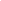
\includegraphics{Images/pixel.png}

%% Back cover
\newpage
\thispagestyle{empty} 
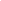
\includegraphics{Images/pixel.png}\\[187mm] 
\vfill
{
\large For Corina server and desktop\\
version \versionnumber\\[4mm]
}




\end{document}
